\documentclass{article}
\textwidth 6.5in \oddsidemargin .06in \evensidemargin .06in
\textheight 8.5in \topmargin -.6in
\PassOptionsToPackage{table}{xcolor}
\usepackage{amsmath}
\usepackage{tikz}

\usepackage{amssymb,latexsym}
\usepackage{amsxtra}
\usepackage{amsthm}
\usepackage{booktabs} % Required for top, mid and bottom rules


\usepackage[ruled, linesnumbered, vlined]{algorithm2e} % algorithm
%\usepackage{xcolor,colortbl}
\usepackage{graphicx}


\usepackage{setspace}
\usepackage{pdfpages}
%\usepackage{verbatim} 
%\usepackage[outputdir=.texpadtmp]{minted}
%\usepackage[skins]{tcolorbox}
%\tcbuselibrary{skins,theorems}
%\tcbuselibrary{breakable}


%----------------------

\usepackage{hyperref}
\hypersetup{
    colorlinks=true,
    linkcolor=black,
    filecolor=magenta,      
    urlcolor=cyan,
    pdftitle={Overleaf Example},
    pdfpagemode=FullScreen,
    }
\urlstyle{same}

\newcommand{\C}[1]{\begin{CJK}{UTF8}{gkai} #1\end{CJK}}


\setlength{\arrayrulewidth}{0.5mm} %This sets the thickness of the borders of the table
%\setlength{\tabcolsep}{18pt}
\renewcommand{\arraystretch}{1.6} 

%-----------------------------------------------------------------------------%
\theoremstyle{definition}
\newtheorem{Definition}{Defintion}
\newtheorem{Theorem}[Definition]{Theorem}
\newtheorem{Example}[Definition]{Example}

\newtheorem{remark}{Remark}[subsection]
\newtheorem{Lemma}{Lemma}[section]
\newtheorem{Corollary}{Corollary}[section]

\newtheorem{Proposition}[Definition]{Proposition}

\linespread{1.5}


\newcommand{\bfw}[1]{\textbf{\textcolor{white}{#1}}}

\newcommand{\df}{\displaystyle \frac} 
\newcommand{\dlim}{\displaystyle \lim}
\newcommand{\dint}{\displaystyle \int}
\newcommand{\ra}{\rangle}
\newcommand{\la}{\langle}
\newcommand{\inner}[2]{{\langle #1,#2\rangle}}
\newcommand{\x}{\mathbf{x}}
\newcommand{\xt}{\mathbf{x}^{\mathsf{T}}}
\newcommand{\T}{{\mathsf{T}}}
\newcommand{\abf}{\mathbf{a}}
\newcommand{\abft}{\mathbf{a}^{\mathsf{T}}}
\newcommand{\R}{\mathbb{R}}
\newcommand{\E}{\mathrm{e}}
\newcommand{\F}{\mathbb{F}}
\newcommand{\X}{\mathbf{X}}
\newcommand{\Y}{\mathbf{Y}}
\newcommand{\y}{\mathbf{y}}
\renewcommand{\l}{\mathcal{l}}

\newcommand{\z}{\mathbf{z}}
\newcommand{\Z}{\mathbf{Z}}
\newcommand{\bfi}{\mathbf{i}}
\newcommand{\bftheta}{\bm{\theta}}
\newcommand{\rmvec}{\mathrm{vec}}
\newcommand{\argmin}{\mathop{\arg\min}}
\newcommand{\argmax}{\mathop{\arg\max}}
\newcommand{\f}{\mathbf{f}}
\newcommand{\U}{\mathbf{u}}
\newcommand{\D}{\mathrm{d}}
\newcommand{\MCG}{\mathcal{G}}
\newcommand{\MCH}{\mathcal{H}}
\newcommand{\MCF}{\mathcal{F}}
\newcommand{\M}{\mathcal{M}}
\newcommand{\W}{\mathbf{W}}
\newcommand{\bfb}{\mathbf{b}}
\newcommand{\MCB}{\mathcal{B}}
\newcommand{\MCT}{\mathcal{T}}
\newcommand{\LL}{\mathcal{L}}
\newcommand{\nullspace}{\mathrm{null}}
\newcommand{\tr}{\mathrm{tr}}
\newcommand{\range}{\mathrm{range}}
\newcommand{\listofalgorithmes}{\tocfile{\listalgorithmcfname}{loa}}
\usepackage{CJK}



\begin{document}
\title{RGBoost: A revised gradient boosting machine
\footnote{Nanyi Zhang is at School of Insurance and Economics, University of International Business and Economics, Beijing 100029, China.
		} }
\author{ Nanyi Zhang\footnote{Corresponding author. Email: nymath@163.com}}
\date{}
\maketitle

\begin{abstract}

This paper presents a novel variant of the gradient boosting algorithm, termed RGBoost, that enhances performance by modifying the negative gradient in every iteration. We begin by offering a precise definition of the gradient, drawing upon the Riesz representation theorem. We then establish that in the conventional gradient boosting algorithm, the gradient vector exhibits bias when the hypothesis space is a Reproducing Kernel Hilbert Space (RKHS). By rectifying this bias, the adjusted gradient vector provides a more accurate approximation of the gradient function. Conclusively, through a series of tests on simulated data, we show that our revised model significantly surpasses the performance of the traditional model.
 \\
{\bf Keywords}: Gradient boosting, Reproducing Kernel Hilbert Space(RKHS), Function Approximation, investment
\end{abstract}

\section{Introduction}
Gradient Boosting Machines (GBMs) are highly effective machine learning algorithms extensively utilized for diverse tasks including regression and classification. They build a robust learner by sequentially amalgamating weak learners, exhibiting remarkable performance across various datasets. Consequently, GBMs have emerged as a highly esteemed model in statistical learning, with the entire process often viewed as a variational method where the functional gradient algorithm strives to optimize the goal function.

The concept of boosting weak learners was first proposed by Freund with Adaboost, followed by Schapire~\cite{freund1996experiments}. Friedman later introduced a gradient boosting-based algorithm~\cite{friedman2001greedy}, and the concept of gradient boosting has since been further developed and expanded. In 2001, Breiman introduced Random Forest, a variant of gradient boosting that combines decision trees and random subspace sampling to enhance the algorithm's performance~\cite{breiman2001random}. Subsequently, Hastie, Tibshirani, and Friedman developed Gradient Boosted Regression Trees (GBRT) in 2006, combining decision trees and gradient boosting to create a powerful and flexible machine learning algorithm for regression problems. In 2015, Chen introduced XGBoost, a widely-used implementation of GBM based on decision trees, employing a novel regularization technique to prevent overfitting~\cite{chen2015xgboost}. XGBoost incorporates advanced features such as parallel processing, distributed computing, and early stopping, and has been widely adopted in both industry and research, winning numerous machine learning competitions.

Microsoft introduced another implementation of GBM, LightGBM, in 2017~\cite{ke2017lightgbm}. LightGBM uses a novel histogram-based approach to accelerate gradient computation and includes advanced features such as categorical feature handling and GPU acceleration. LightGBM has been shown to outperform other popular gradient-boosting algorithms in terms of speed and accuracy. These related works have significantly advanced the field of gradient boosting, making it a popular and powerful machine learning technique.

Traditional boosting algorithms often use decision trees as base learners due to their simplicity. However, there is no restriction on the type of base learners that can be employed. The gradient boosting algorithm can be viewed as an approximated functional gradient descent process, wherein a base learner is chosen to approximate the gradient function queried at $(x_1, \cdots, x_n)$ in the $L^2$ norm.

Many studies have focused on choosing different types of base learners, such as Generalized Linear Models (GLMs), Kernel functions, splines, and others. Some research has also attempted to combine different base learners within the boosting framework. For example, Sigrist~\cite{sigrist2021ktboost} and Hoffmann~\cite{hoffmann2004combining} achieved lower bias and error by combining various base learners.

Nonetheless, limited research has been conducted on modifying the negative gradient vector, a critical element in each iteration. We argue that the negative gradient vector used by Friedman~\cite{friedman2001greedy} is biased and propose a superior alternative by assuming the hypothesis space is a Reproducing Kernel Hilbert Space (RKHS).

To validate our model's effectiveness, we first introduce the concept of Fréchet derivatives, essential in functional analysis. We then examine the differential of functionals in function space, playing a crucial role in mathematical analysis. By providing a clear definition of the gradient using the Riesz representation theorem, we establish a rigorous framework for understanding the concept of the gradient in functional spaces. Next, by employing the chain rule of Fréchet derivatives, we calculate the gradient of the empirical loss function and embed it into the boosting algorithm. Finally, simulated data verifies our model's accuracy, with the revised model exhibiting a faster convergence rate and smaller test error.

The remainder of this paper is organized as follows: Section 2 introduces functional analysis concepts and derives an alternative negative gradient vector. We then discuss the regression range and determine which function our model will approximate. In Section 3, we design the gradient boosting machine and introduce the \texttt{rgboost} package in Python. Section 4 presents a series of experiments on simulated data to validate our model's effectiveness.Lastly, Section 5 concludes the paper and highlights its contributions to the field of gradient boosting.
\section{The model}
In this section, we explore foundational concepts in functional analysis and refine the definition of the gradient using the Riesz Representation Theorem. We then compute the gradient of the empirical loss functional under the assumption that the hypothesis space is a Reproducing Kernel Hilbert Space (RKHS). Our analysis uncovers a bias in the gradient estimation step of Friedman's boosting algorithm. To rectify this bias, we propose using the vector, derived from evaluating the gradient function at sample points, as the negative gradient vector in our boosting algorithm.

The objective of a gradient-boosting machine is to pinpoint an element within the hypothesis space that minimizes the empirical loss function. This goal is typically achieved via a gradient descent algorithm that operates within a functional space. However, performing gradient descent in such a space requires the use of more advanced mathematical tools. Thus, we initiate this section by presenting the necessary preliminaries in functional analysis.



\subsection{Preliminaries}

To provide a more detailed description of our model, we first introduce some notions in functional analysis.
Let $\mathcal{H}$ be a vector space. We define the evaluation functional $E_x$ as the function that maps a functional in $\mathcal{H}$ to its function value at $x$. Specifically, let
\begin{equation}\label{eq:eval-functional}
E_x: \mathcal{H} \to \R, \quad f \mapsto f(x).
\end{equation}

Observe that $E_x(f+g) = (f+g)(x) = E_x(f) + E_x(g)$, which implies that $E_x$ is a linear functional on $\mathcal{H}$.

In Equation \ref{eq:eval-functional}, we use the notation $\mathcal{H}$ to represent a function space because $\mathcal{H}$ often stands for the hypothesis space or the Hilbert space. A Hilbert space is a complete inner product space. The norm measures the distance between vectors, while the inner product can describe the correlation between two elements in a space. Since we need to discuss certain analytic properties, such as continuity, differentiability, or general limits, we require a complete space in which every Cauchy sequence has a limit. This is where a Hilbert space comes into play. It combines the aforementioned requirements and is thus widely used in this context.

Another crucial concept is the Frechet derivative. The Frechet derivative is a method to extend the derivative to function spaces. It measures the rate of change of a functional under small perturbations of its arguments. The Fréchet derivative is defined as the best linear approximation of the functional at a given point. Specifically, we define the Fréchet derivative of $f$ as a map from $\mathcal{X}$ to a linear functional $D_{f,x}$ on $\mathcal{X}$,
$$
D_{f}: \mathrm{int}_{\mathcal{X}} \to B(\mathcal{X},\mathcal{Y}), \quad x \mapsto D_{f,x}.
$$
To get an insight into $D_f$, we take a multivariate function as an example. In calculus, we have that. 
$$
D_{f,x_0} = \sum_{i=1}^n \partial f_i (x_o) \D x_i.
$$
%\begin{Example}
%Suppose $f: \R^n \to \R$, the frechet deritive of $f$ at $x_0$ is 
%
%\begin{eqnarray*}
%D_{f,x_0} &=& \sum_{i=1}^n \partial_i f (x_0) \D x_i \\
%&=& \mathbf{J}_f^x \D \x
%\end{eqnarray*}
%\end{Example}
Where
$$
\D x_i : \R^n \to \R, \quad h \mapsto h_i.
$$
Note that $\D x_i$ is the dual bases on $\R^n$ with respect to standard normal basis, since
$$
\D x_i (e_j) = \delta_{ij}.
$$

%\begin{Example}
%Suppose $f: \R^n \to \R^m$, then the frechet of $f$ at $x_0$ is 
%\end{Example}

%
%\begin{Proposition}[Rules of differentiation] \ \\
%\begin{itemize}
%	\item $D_{af,x} = a D_{f,x}.$
%	\item $D_{f+g,x} = D_{f,x} + D_{g,x}$
%	\item $D_{fg,x} = g(x)D_{f,x} + f(x)D_{g,x}$
%\end{itemize}
%\end{Proposition}
%
%\begin{Proposition}[The Chain Rule] \ \\
%Let X,Y and Z be normed vector spaces. Let $f: X \to Y$ and $g: Y \to Z$ are two maps such that $f$ is frechet differentiable at $x \in \mathrm{int}_X$ and $g$ at $f(x) \in \mathrm{int}_Y.$ Then, $g \circ f$ is frechet differentiable at $x$, and
%\begin{equation}\label{thm:ChainRule}
%	D_{g \circ f},x = D_{g,f(x)} \circ D_{f,x}
%\end{equation}
%\end{Proposition}
%\begin{proof}
%$$
%f(\omega+x) - f(x) = D_{f,x}(w) + \E_{f,x}(\omega)
%$$
%
%In addition,
%$$
%g(\omega+f(x))- g(f(x)) = D_{g,f(x)}(\omega) + \E_{g,f(x)}(\omega).
%$$
%thus
%
%\begin{eqnarray*}
%g(f(\omega+x))-g(f(x)) &=& D_{g,f(x)}(f(\omega+x)-f(x)) + \E_{g,f(x)}(f(\omega)) \\
%&=& D_{g,f(x)}( D_{f,x}(\omega)) + D_{g,f(x)}(\E_{f,x}(\omega)) + \E_{g,f(x)} \\
%&=& (D_{g,f(x)} \circ D_{f,x})(\omega) + \E_{g\circ f,x}(\omega).                                                                                                                                                                                                                                                                                                                                                                                                                  
%\end{eqnarray*}
%
%\end{proof}


%\begin{Proposition}[Differentiation of inverse function] \ \\
%Suppose $V$ is normed vector space and $f: V \to V$. Then
%$$
%D_{f^{-1},x} = (D_{f,f^{-1}(x)})^{-1} \circ D_{I,x},
%$$
%where 
%$$
%(D_{f,f^{-1}(x)})^{-1}(a) = (\mathrm{J}_f^{f^{-1}(x)})^{-1} a.
%$$
%\end{Proposition}



Next, we will introduce a widely used theorem for understanding function spaces' structure. This theorem has many applications in mathematics, physics, and even economics. For example, the Riesz representation theorem in finance implies that a payoff can represent any linear functional on the asset span.

\begin{Theorem}[Riesz Representation Theorem] \ \\ 
Suppose $\varphi$ is a bounded linear functional on a Hilbert space $V$. Then there exists a unique $h \in V$ such that
$$
\varphi(f) = \inner{f}{h}, \quad f \in \mathcal{H}.
$$
\end{Theorem}
The Riesz Representation Theorem is a cornerstone in functional analysis, establishing a one-to-one correspondence between linear functionals on a Hilbert space and the elements within that space. Specifically, it stipulates that for any bounded linear functional $f$ on a Hilbert space $\mathcal{H}$, there exists a unique element $h$ in $\mathcal{H}$ such that $\varphi(f) = \langle f, h\rangle$ for all $f$ in $\mathcal{H}$. Here, $\langle\cdot,\cdot\rangle$ denotes the inner product on $\mathcal{H}$.

In a complete normed vector space, the continuity of a linear functional is equivalent to its boundedness. Given the essential role of the evaluation functional in our model, we require a more suitable space to explore it. It's important to note that not all evaluation functionals of a Hilbert space are bounded. To satisfy the Riesz Representation Theorem's requirements, we define the Reproducing Kernel Hilbert Space (RKHS) as a space wherein every evaluation function is bounded, even though they may not consistently be so.

\begin{Definition}[RKHS] \ \\
	Let $X$ be a set and $\mathcal{H}$ a Hilbert space with $\mathcal{H} \subset \R^{X}$. If the evaluation functional $E_x$ over $\mathcal{H}$ is bounded. (or equivalently, continuous), then we say $\mathcal{H}$ is a Reproducing Kernel Hilbert Space.
\end{Definition}

Since the evaluation functional on $\mathcal{H}$ is bounded, the Riesz Representation Theorem suggests that there exists a unique vector $K_x \in \mathcal{H}$ which satisfies the following  
$$
f(x) = E_x(f) = \inner{f}{K_x}_{\mathcal{H}}.
$$
Also 
$$
K_x(y) = E_y(K_x) = \inner{K_x}{K_y}_{\mathcal{H}}.
$$
This allows us to define the reproducing kernel of $\mathcal{H}$ as a function. 
$$
K: X \times X \to \R, \quad (x,y) \mapsto K(x,y) = \inner{K_x}{K_y}_{\mathcal{H}}.
$$
\C{}
However, in practical applications, confirming whether the evaluation functional in a Hilbert space is bounded can be challenging. Even if it is bounded, the Riesz representation theorem only informs us of the existence of a kernel but does not give the analytic expression of the kernel. As a result, we commonly rely on a symmetric and positive definite function to construct a Hilbert space, known as the Moore-Aronszajn theorem.

\begin{Theorem}[Moore-Aronszajn] \ \\
Suppose $K$ is a symmetric positive definitive function on $X \times X$. Then there is a unique Hilbert Space of functions on $X$ for which $K$ is a reproducing Kernel.
	
\end{Theorem}

Next, we will give a better definition of the gradient. First, recall the definition of the gradient in calculus. It is a vector that points in the direction of the steepest increase of the function at a particular point. It can be calculated by taking the partial derivative with respect to each coordinate. The inner product of a gradient and the increment can be viewed as the linear approximation of the increment of the function value. This idea can be directly extended to a function space. Specifically, suppose $\MCH$ is a normed vector space, and $L$ is a function defined at $x_0 \in \MCH$. We know that $L$ is Frechet differentiable on $\MCH$ if and only if 
\begin{equation} \label{frechet}
	L(x_0 + h) = L(x_0) + D_{L,x_0}(h) + e_{x_0}(h), \quad \forall h \in \mathcal{H}.
\end{equation}

Where $D_{L,x_0}$ is a linear functional on $\MCH$ and the error part must moves faster to zero than $h$, that is 
$$\lim_{h \to 0} \frac{e_{x_0} (h)}{\Vert h \Vert} = 0.$$
Note that the zero on the right side of the above equation is the additive identity($0: \mathcal{H} \to \R,\quad f \mapsto 0$) in $\mathcal{H}$ rather than the real number $0$.

Now, the Riesz Representation Theorem ensures a unique vector $g(x_0,L) \in \mathcal{H}$ exists and has the following property:
$$
D_{L,x_0}(h) = \inner{h}{g(x_0,L)}.
$$ 
This reminds us to define the gradient of function as the unique element in the Hypothesis space that represents the Frechet derivative of the functional.

%\begin{Definition}{The gradient of a real function}
%	
%\end{Definition}
Suppose $f$ is a multivariate function; according to our definition, the gradient of 
$f$ at $x_0$ is the Jacobian matrix of $f$ as $x_0$.
$$
\nabla f(x_0) = \mathbf{J}_f^{x_0}=(\partial_1 f(x_0), \cdots, \partial_n f(x_0)) .
$$
Next we introduce the gradient of evaluation functional.
\begin{Theorem}[Gradient of the evaluation functional] \label{EVAL}\ \\ 
Suppose $\MCH$ is an RKHS. Then the gradient of the evaluation functional at $f$ when given x is 
$$
\nabla E_x (f) = K_x \in \mathcal{H}.
$$
\end{Theorem}
\begin{proof}

\begin{eqnarray*}
E_x(f + h) &=& E_x(f) + E_x(h) \\
&=& E_x(f) + \inner{K_x}{h} + 0. \\ 
\end{eqnarray*}
The Riesz Representation theorem admits the uniqueness of $K_x$.
\end{proof}
Suppose $\Vert h \Vert =1$, we have the following:
\begin{eqnarray*}
L(f_0+h) - L(f_0) &\sim& \langle \nabla L (f_0), h \rangle \\
& \geq & -\Vert \nabla L (f_0) \Vert.
\end{eqnarray*}

This provides a  way to find the local minimum of a functional. Indeed, 
the equation above suggests that $L$ moves the fastest when walking along the gradient's direction, thus giving us an idea to minimize a functional. We state this in Algorithm 1.

\begin{center}
\begin{minipage}{0.95\linewidth}
\begin{algorithm}[H]
\setstretch{1.5}
\SetAlgoLined
\caption{Function Gradient descend algorithm}
\KwIn{\begin{itemize}
	\item the functinal $L: V \to \R$.
	\item number of iterations $M \geq 1$
	\item leanring rate $\eta \in (0,1]$
\end{itemize}
}
Initialize $f_0$ \\
\While{$m \in \{1,\cdots,M\}$}{
Calculate the gradient: 
$$
\nabla L (f_{m-1}) 
$$

Find the best gradient descent step-size: 
$$
\rho_m = \argmin_{\rho \in \R} L (f_{m-1} - \rho \nabla L (f_{m-1})))
$$

Update: $$f_m \gets f_{m-1} - \eta \rho_m \nabla L (f_{m-1})$$
}
\KwOut{$f_M$}
\end{algorithm}
\end{minipage}
\end{center}

Algorithm 1 is a powerful tool for solving some variational problems. At each iteration, we first calculate the gradient of loss functional and then find the best gradient descent step size using linear search. However, calculating the gradient of a functional raises a problem since the Riesz representation theorem can only ensure the existence of a gradient. 
One solution is to find an element in the hypothesis space as close to the gradient as possible. 

Since the gradient function can only be observed at finite sample points, we focus on the empirical case. Our goal is to find the local minimum of $\LL$, where
\begin{equation}\label{eq:EmpiricalLoss} \LL: \mathcal{H} \to \R, \quad f \mapsto \frac{1}{n} \sum_{i=1}^n L(y_i, f(x_i)). \end{equation}
Before starting the gradient descent algorithm, we define another functional $\LL^\prime$, which is derived from $\LL$:
\begin{equation} \LL^\prime: \R^n \to \R, \quad h \mapsto \frac{1}{n} \sum_{i=1}^n L(y_i, h_i), \end{equation}
where $h_i$ represents the i-th coordinate of vector $h$.
Next, we will examine the relationship between $\LL$ and $\LL^\prime$. To simplify the notation, let $\hat y = (f(x_1),\cdots, f(x_n))^T$. By definition, we have $\LL(f) = \LL^\prime(\hat y)$. Now, we will calculate the gradients of $\LL$ and $\LL^\prime$.


\begin{equation}\label{gradient_LLP}
\nabla \LL^\prime (\hat y) = \begin{bmatrix}
	 \frac{1}{n} \partial_2 L (y_1, f(x_1)) \\ 
	 \frac{1}{n} \partial_2 L (y_2, f(x_2)) \\ 
	\vdots \\
	 \frac{1}{n} \partial_2 L (y_n, f(x_n)) \\ 
\end{bmatrix}
\end{equation}


With knowledge of calculus, the gradient of a multivariate function is composed of partial derivatives, as shown in Equation (\ref{gradient_LLP}). The negative gradient vector in Friedman's boosting algorithm is represented by $\nabla \LL^\prime (\hat y)$. Algorithm 2 outlines the implementation of this algorithm. Note that $\partial_2 L$ refers to the partial derivative of the second component.

\begin{center}

\begin{minipage}{0.95\linewidth}
\begin{algorithm}[H]
\setstretch{1.5}
\SetAlgoLined
\caption{Friedman's Gradient Boosting algorithm}
\KwIn{\begin{itemize}
	\vspace{-0.3cm}
	\item the functinal $L: V \to \R$.
	\vspace{-0.4cm}
	\item number of iterations $M \geq 1$
	\vspace{-0.4cm}
	\item leanring rate $\eta \in (0,1]$
\end{itemize}
}
\vspace{-0.4cm}
Initialize $F_0 =\arg \min _\rho \sum_{i=1}^n L\left(y_i, \rho\right)$ \\
\While{$m \in \{1,\cdots,M\}$}{
Calculate the negative gradient: 
$$
g_{m,i}=-\left[\frac{\partial L\left(y_i, F\left(\mathbf{x}_i\right)\right)}{\partial F\left(\mathbf{x}_i\right)}\right]_{F(\mathbf{x})=F_{m-1}(\mathbf{x})},\  i=1, \cdots,n
$$ \\
\vspace{-0.3cm}
Fit a base estimator:
$$
\mathbf{a}_m=\arg \min _{\mathbf{a}, \beta} \sum_{i=1}^n\left[g_{m,i}-\beta h\left(\mathbf{x}_i ; \mathbf{a}\right)\right]^2
$$ \\
\vspace{-0.3cm}
Find the best gradient descent step-size: 
\vspace{-.3cm}
$$
\rho_m=\arg \min _\rho \sum_{i=1}^n L\left(y_i, F_{m-1}\left(\mathbf{x}_i\right)+\rho h\left(\mathbf{x}_i ; \mathbf{a}_m\right)\right)
$$ \\
\vspace{-.5cm}
Update: $$F_m(\mathbf{x})=F_{m-1}(\mathbf{x})+\rho_m h\left(\mathbf{x} ; \mathbf{a}_m\right)$$
}
\KwOut{$F_M$}
\end{algorithm}
\end{minipage}
\end{center}

In order to maintain consistency with our model's notation, we will list the algorithm without changing any symbols. However, note that the notation $\frac{\partial L\left(y_i, F\left(\mathbf{x}_i\right)\right)}{\partial F\left(\mathbf{x}_i\right)}$ is equivalent to $\partial_2L(y_i, F(x_i))$.

In step 4 of the algorithm, a base learner is chosen to fit the gradient vector in $L^2$ norm at sample points. This learner can be viesw as the gradient function in algorithm 1.


\subsection{The revised gradient boosting machine}
In this part of the section, we unveil our revised model. It is crucial to note that the negative gradient vector in Algorithm 2 signifies the gradient of the derived empirical loss functional $\mathcal{L}^\prime$, not the gradient of $\mathcal{L}$. Although calculating the gradient of the empirical loss functional $\mathcal{L}$ at $f$ may seem daunting, Theorem \ref{EVAL} provides an explicit expression for it.

\begin{Theorem}[The gradient of empirical loss function] \label{thm:gradient-of-LL}\ \\
Suppose $\mathcal{H}$ is a RKHS with kernel $K$ defined on it. Then the gradient of the empirical loss function $\mathcal{L}$ can be expressed as
$$
\nabla \LL (f) = \frac{1}{n} \sum_{i=1}^{n} \partial_2 L(y_i,f(x_i)) K_{x_i}. 
$$
\end{Theorem}
\begin{proof}
The proof can be found in the Appendix A.
\end{proof}


Here $\nabla \LL (f)$ is a functional on $\mathcal{X}$ and it can only be observed at finite sample points. For example 
$$
\nabla \LL (f) (x_1) = \frac{1}{n} \sum_{i=1}^{n} \partial_2 L(y_i,f(x_i)) K(x_i, x_1) .
$$ 
And we have the following relationship,

\begin{eqnarray*}
\begin{bmatrix}
\nabla \mathcal{L}(f)(x_1) \\
\vdots \\
\nabla \mathcal{L}(f)(x_n) 
\end{bmatrix}
& = & \begin{bmatrix}
	 \frac{1}{n} \partial_2 L (y_1, f(x_1)), &
	\cdots, &
	 \frac{1}{n} \partial_2 L (y_n, f(x_n)) 
\end{bmatrix} \begin{bmatrix}
	K(x_1,x_1)  & \cdots & K(x_1,x_n) \\
	\vdots  & & \vdots \\
	K(x_n,x_1)  & \cdots & K(x_n,x_n) \\	
\end{bmatrix}\\
& = &(\nabla \LL^\prime (\hat y))^T K.
\end{eqnarray*} \\


We now claim that $\nabla \LL^\prime (\hat y)$ is not always equal to the gradient function $\nabla \LL (f)$ which evaluated at sample points. In fact, they are the same if and only if 
$$
K(x_i,x_j) = \chi_{\{x_i\}}(x_j) = \delta_{ij},
$$
where $\chi$ is the characteristic functional of set. Based on the result of theorem \ref{thm:gradient-of-LL}, we revise the step 3 in Friedman's gradient boosting algorithm in algorithm 3.

\begin{center}
\begin{minipage}{0.95\linewidth}
\begin{algorithm}[H]
\setstretch{1.5}
\SetAlgoLined
\caption{The Revised Gradient boosting algorithm}
\KwData{$\mathcal{D}=\{(y_1,x_1),\cdots,(y_n,x_n)\}$}
\KwIn{\begin{itemize}
	\vspace{-.3cm}
	\item the hypothesis $\mathcal{H}$ and the reproducing kernel $K$.
	\vspace{-.3cm}
	\item the empirical loss function $\mathcal{L}: \mathcal{H} \to \R$
	\vspace{-.3cm}
	\item number of iterations $M \geq 1$
	\vspace{-.3cm}
	\item leanring rate $\eta \in (0,1]$
\end{itemize}
}
\vspace{-.3cm}
Initialize $f_0, \quad f_0(x) = \argmin_{c \in \R} \frac{1}{n} \sum_{i=1}^nL(y_i,c)$ for all $x \in \R^p.$\\
\While{$m \in \{1,\cdots,M\}$}{
Calculate the negative gradient vector: 
\vspace{-.3cm}
$$
g_{m,j} = -\frac{1}{n}\sum_{i=1}^n \partial_2 L(y_i, f_{m-1}(x_i))K(x_i,x_j), \quad j = 1,2, \cdots, n.
\vspace{-.3cm} 
$$\\
Fit the gradient vector: 
\vspace{-.1cm}
$$
h_m = \argmin_{h \in \mathcal{H},\beta} \sum_{i=1}^n (g_{m,i} - \beta h_m(x_i))^2
\vspace{-.1cm}
$$  \\
Find the best gradient descent step-size: 
\vspace{-.3cm}
$$
\rho_m = \argmin_{\rho \in \R} \mathcal{L}(f_{m-1} + \rho h_m)
\vspace{-.3cm}
$$ \\
Update: $$f_m \gets f_{m-1} + \eta \rho_m h_m$$
}
\KwOut{$f_M = f_0 + \sum_{i=1}^M \eta \rho_m h_m$}
\end{algorithm}
\end{minipage}
\end{center}

Algorithm 3 is a revised version of the gradient boosting machine. In Step 1, we search for a constant function that minimizes the empirical loss function. If we apply the square loss function, this constant must be the sample mean of $y$. In Step 3, we substitute the gradient based on Theorem \ref{thm:gradient-of-LL}.


%\subsection{Connections with other boosting algorithm}
%
%\begin{Theorem}(Adaboost) \ \\
%Suppose the loss function is $L(y, \hat y) = \E^{-y\hat y}$, and the Gram matrix is the identity matrix then todo.
%\end{Theorem}
%\begin{proof}
%\begin{eqnarray*}
%	g_{m,j} = -\frac{1}{n} y_i \E^{-y_j(f_{m-1}(x_j))}
%\end{eqnarray*}
%\end{proof}

\subsection{Statistical theory of regression}
This subsection delves into the statistical theory underpinning regression. As previously highlighted, gradient boosting machines (GBM) serve as an approximation tool for the function minimizing the empirical loss function. Thus, the choice of the loss function and function to be approximated warrants discussion. We elucidate the statistical theory of regression, demonstrating that GBM can approximate the conditional expectation function $m(x) = E(Y|X=x)$ using the $L^2$ loss function.

To elucidate these concepts, we examine them within the context of measure theory. We commence with a measurable space, comprising a set and a sigma-algebra defined on it. A measure, a set function adhering to countable additivity, can be established on this measurable space. Integration with respect to measure boasts superior attributes compared to Riemann integration encountered in calculus. Despite the intuitiveness of Riemann integration, it loses its effectiveness when the function is defined in an abstract space. Conversely, Lebesgue integration overcomes these limitations, offering numerous advantages over Riemann integration. Its primary strength lies in its generality, as it accommodates a broader set of functions, including those not Riemann integrable. Lebesgue integration is also more flexible, allowing for the integration of functions with respect to more diverse measures, not just the Lebesgue measure. Its superior convergence properties compared to Riemann integration further enhance its appeal, making it especially apt for various analysis and probability theory applications. The integration of a random variable with respect to a probability measure bears a relationship with Lebesgue-Stieltjes integration.

%\begin{Definition}{Measurable Map} \ \\
%Suppose $(\Omega, \MCF)$ and $(E, \mathcal{E})$ are both measurable spaces. A map 
%$$
%f: \Omega \to E
%$$
%is called $\MCF$- measurable if 
%$$
%\forall A \in \mathcal{E},\quad f^{-1}(A) = \{\omega \in \Omega: f(\omega) \in A \} \in \MCF.
%$$
%\end{Definition}
%
%
%\begin{Theorem}{} \ \\
%We define the inverse of a sigma-algebra as the collection of sets in the form of 
%$$
%f^{-1}(\mathcal{E}) := \{ f^{-1}(A): A \in \mathcal{E} \}.
%$$
%Then $f$ is $\mathcal{F}$-measurable if and only if 
%$f^{-1}(\mathcal{E})$ is a sigma-algebra. 
%
%\end{Theorem}
%
%\begin{Theorem}{} \ \\
%Suppose $P$ is a measure on $(\Omega, \mathcal{F})$ and $f \in \M(\MCF)$, then the function induced $f$
%$$
%\mu_{f} = P \circ f^{-1}
%$$
%is a measure on $(E, \mathcal{E})$. 
%\end{Theorem}
%In probability theory, $\mu_f$ is often called the distribution function of $f$.




\begin{Theorem}[Measure transformations]\label{thm:LS-to-RS} \ \\
Suppose $(\Omega, \mathcal{F})$ and $(E, \mathcal{E})$ are two measurable spaces, $f: \Omega \to E$, $g: E \to \R$. Then we have the following
\begin{eqnarray}\label{thm:changeofmeasure}
\int_\Omega g \circ f \D P = \int_E  g \circ I \D \mu_f,
\end{eqnarray}
where $I: E \to E, x \mapsto x$.
\end{Theorem}
\begin{proof}
The proof can be found in the Appendix.
\end{proof}

Theorem \ref{thm:LS-to-RS} has many applications in probability theory. For example, we can calculate the expectation of $g(X)$ by using the formula $E(g(X)) = \int_\R g(x) \D F_X(x).$

The objective of regression is to identify the conditional expectation function, which is a key concept in probability theory and statistics. It represents the anticipated value of a random variable based on certain information provided by  another random variable. Appendix B provides a definition of conditional expectation, as well as its properties. According to the following theorem, the conditional expectation with respect to a sigma-algebra generated by a random map can be expressed as a borel-measurable function composition of this random map.
\begin{Theorem}\label{thm:cond1}
Suppose $X: \Omega \to \R^p$, X is random vevtor, then there exists a borel-measurable function f $\R^p \to \R$, such that
$$
E(Y|\sigma(X)) = f \circ X
$$
\end{Theorem}
\begin{proof}
The proof can be found in Appendix A.
\end{proof}
The converse of Theorem \ref{thm:cond1} is also true, and it provides an efficient method for calculating the conditional expectation function so long as the sigma algebra is generated by a random map, since $E(Y|X=x)$ can often be easily obtained.

\begin{Theorem}[The connection between different types of contional expectations] \label{thm:relationship} \ \\
Suppose $m: \R^p \to \R, \quad x \mapsto E(Y|X=x)$ is a borel-measurable function, then
\begin{equation}
m \circ X = E(Y|\sigma(X)).
\end{equation}
\end{Theorem}
\begin{proof}
The proof can be found in Appendix A.
\end{proof}


To gain a deeper understanding of conditional expectation and regression, we relax the restrictions on $Y$ slightly. Specifically, we assume that $Y \in \mathcal{L}^2(\Omega, \mathcal{F}, P)$ and $\mathcal{G}$ is a sub-sigma-algebra of $\mathcal{F}$. We can then consider the space $\mathcal{L}^2(\Omega, \mathcal{G}, P_{\mathcal{G}})$, which is a closed subspace of $\mathcal{L}^2(\Omega, \mathcal{F}, P)$. According to the Hilbert project theorem, there exists a unique element $M$ in $\mathcal{L}^2(\Omega, \mathcal{G}, P_{\mathcal{G}})$ such that
\begin{equation}
\Vert Y - M \Vert_2 \leq \Vert Y- f\Vert_2, \quad \forall f \in \mathcal{L}^2(\Omega, \mathcal{G}, P_{\mathcal{G}}),	
\end{equation}
and
$$
Y - M \perp f, \quad \forall f \in \mathcal{L}^2(\Omega, \mathcal{G}, P_{\mathcal{G}}).
$$
The partial average of $M$ is equal to that of $Y$, making it sufficient to serve as a conditional expectation. In this sense, we can see the conditional expectation as a projection onto the subspace created by $\mathcal{G}$. Figure \ref{fig:conditonalexpectation} reveals the relationship of $Y$, $E(Y|\mathcal{G})$ and $E(Y)$. Note that the variance decomposition formula is the Pythagoras theorem in a Hilbert space.
\begin{equation}
	Var(Y) = Var(E(Y|X))+ E(Var(Y|X)).
\end{equation}
\begin{figure}[htb]
	\centering
	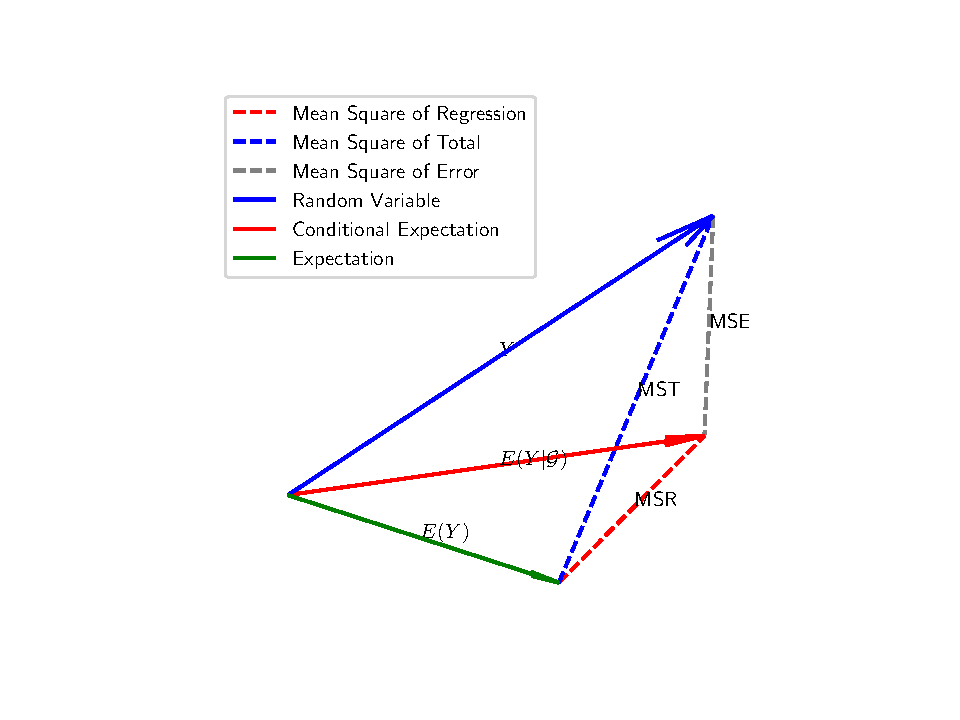
\includegraphics{figure/conditional.pdf}
	\vspace{-1.7cm}
	\caption{Conditional Expectation as a projection.}
	\label{fig:conditonalexpectation}
\end{figure}

The regression model can be structed as follows, suppose we have a random variable $Y$ defined on a probability space $(\Omega, \mathcal{F}, P)$, and a random map $X$ from $\Omega$ to a vector space $E$ (often denoted as $\R^p$). We can express $Y$ as the sum of its conditional expectation $E(Y|X)$ and the error term $Y-E(Y|X)$, which can be written as $m\circ X + \varepsilon$.

To estimate the conditional expectation from sample data, we need to minimize the empirical loss function:
$$
\argmin_{f \in \mathcal{H}} \frac{1}{n} \sum_{i=1}^n (y_i - f(x_i))^2,
$$

where $y_i$ is the value of $Y$ and $x_i$ is the value of $X$ in the $i$-th sample, and $\mathcal{H}$ is a suitable class of functions. The goal is to find a function $f$ that minimizes the difference between the predicted values and the actual values, as measured by the mean squared error.


There are many ways to optimize the empirical loss function. One of the simplest ways is to parameterize it. For instance, we can set the form of the hypothesis as follows:

There are various methods to optimize the empirical loss function. One of the simplest ways is to parameterize it. For example, we can define the form of the hypothesis as follows:
\begin{equation}
\mathcal{H} = \left\{f: \R^p \to \R, \quad x \mapsto c+ \beta^T x| \text{where}\ \beta \in \R^p, c \in \R \right\}.	
\end{equation}
In this case, the problem can be converted to:
$$
\argmin_{\beta \in \R^{p+1}} \frac{1}{n} \sum_{i=1}^n (y_i - \beta^T \tilde x_i)^2,
$$
where $\mathcal{H}$ is often referred to as the collection of affine functions, and the $\beta$ that minimize the square loss is
$$
\hat \beta = (X^T X)^{-1} X^T Y.
$$
The hypothesis space can also be represented as a reproducing kernel Hilbert space (RKHS). Assuming that $K: \R^p \times \R^p \to \R$ is a positive definite kernel function, there exists an inner product in $\mathcal{H}$ such that $K_x$ belongs to $\mathcal{H}$ for all $x\in \R^p$. According to the representer theorem \cite{scholkopf2001generalized}, there is a unique minimizer in the form of
$$
f = \sum_{i=1}^n \alpha_i K_{x_i}
$$
Moreover, the GLM can be utilized as a Hypothesis. In this scenario, $\mathcal{H}$ can be expressed as follows:
\begin{equation}
\mathcal{H} = \left\{f: \R^p \to \R, \quad x \mapsto g^{-1} \circ(c+ \beta^T x)| \text{where}\ \beta \in \R^p, c \in \R \right\},	
\end{equation}


Here, $g^{-1}$ refers to the inverse of the canonical link function and varies for different cases.


\begin{table}[htb]
\centering
\caption{The Canonical Link Function of GED.}
\vspace{.2cm}
\begin{tabular}{c c c}
\toprule
Distribution &Mean Function & Canonical Link Function \\
\midrule
$N(\mu,\sigma^2)$ & $b^\prime: \theta \mapsto \theta$ & $g: \mu \mapsto \mu$ \\
$Pois(\lambda)$ & $b^\prime: \theta \mapsto \E^{\theta}$& $g: \mu \mapsto \ln \mu$\\
$Bin(1,p)$ & $b^\prime: \theta \mapsto \frac{1}{1+\E^{-\theta}}$ & $g: \mu \mapsto \ln \frac{\mu}{1-\mu}$ \\
\bottomrule
\end{tabular} 
\label{tab:GLM}
\end{table}
















\section{GBM Design}
In this section, we will list the alternative loss functions and base learners, and explain when they can be used. Later, we will discuss some improvement approaches to GBM, such as combining different types of base learners, regularization, subsampling, and others. For more information about the design of GBM, we refer  to NateKin \cite{natekin2013gradient}.

To create a GBM for a particular task, it's important to choose the appropriate options for the empirical loss function $\mathcal{L}$ and the hypothesis $\mathcal{H}$ (which is the set of collections of base learners), because these choices have a significant impact on the GBM's performance. (As we discussed in the previous section, the conditional expectation function minimizes the $L^2$ loss.)


\subsection{Loss functions}
The loss function is a critical element of the gradient boosting machine, as it quantifies the discrepancy between the anticipated and actual values of the target variable. The selection of loss functions (functionals) depends on the objective of our model. For instance, if the goal is to obtain the conditional expectation of the response given $X$, the square loss function ($L^2$ loss) is preferable since the conditional expectation can be considered as the projection of the response, thus attaining the smallest $L^2$ distance to the response. To use a loss function in practice, one must specify both the loss and the corresponding negative gradient. (In our Python module, the loss function is defined as an abstract class with attributes "loss" and "negative gradient".) Other loss functions are provided in Schmid et al., 2011 \cite{schmid2011geoadditive}.

The types of loss functions can be roughly divided according to the type of response
as follows:
\begin{enumerate}
	\item \textbf{Continuous response:}
	\begin{itemize}
		\vspace{-.2cm}
		\item $L^2$ loss (Conditional Expectation)
		\vspace{-.2cm}
		\item $L^1$ loss (Conditional Median)
		\vspace{-.2cm}
		\item Quantile loss (Conditional Quantile)
		\vspace{-.2cm}
		\item ZeroOne loss (Conditional Mode).
		\vspace{-.2cm}
	\end{itemize}
	\item \textbf{Categorical response:}
	\begin{itemize}
		\vspace{-.2cm}
		\item Exponential loss
		\vspace{-.2cm}
		\item Cross-Entropy loss
		\vspace{-.2cm}
	\end{itemize}
	\item \textbf{Other response:}
	\begin{itemize}
		\vspace{-.2cm}
		\item MLE loss 
		\vspace{-.2cm}
		\item Custom loss
		\vspace{-.2cm}
	\end{itemize}
\end{enumerate}

%\begin{table}[htb]
%\centering
%\begin{tabular}{lcc}
%\toprule
%\textbf{Loss Function} & \textbf{Expression} & \textbf{Roles} \\
%\midrule
%$L^2$ Loss& $\frac{1}{2}(y-f)^2$ & conditional expectation \\
%ZeroOne Loss & $I\{y=f\}$ & conditional mode \\
%Exponential Loss & $\exp{(-yf)}$& weight redistribution \\
%CrossEntropy Loss& &   \\
%\bottomrule
%\end{tabular}
%\caption{Loss Functions}
%\label{tab:topmidbottom}
%\end{table}
The framework allows for the use of custom loss functions. One example of their application is in quantitative finance and investment analysis, particularly in stock selection. At each rebalance date, we have a multitude of factors denoted by $F_t \in \R^{m \times N}$, where $m$ is the number of factors and $N$ is the number of stocks. These factors include historical prices, financial ratios, and technical indicators. Our goal is to combine these factors into a vector $\alpha_t \in \R^N$ and then use a given strategy to obtain indicators like Sharpe ratio or excess alpha of future retures. This  can be viewed as a custom loss function.Specifically, we can represent the result at time $t$ as 
\begin{eqnarray*}
\mathrm{result}_t &=& \mathrm{Strategy}_t \circ f \circ F_t \\
 &=&\mathrm{Strategy}_t \circ \alpha_t.
\end{eqnarray*}
In this situation, the custom loss functional can be expressed as 
$$
\mathcal{L}: \mathcal{H} \to \R, \quad f \mapsto \frac{1}{T}\sum_{i=1}^T \mathrm{Strategy}_t \circ f \circ F_t.
$$
Here we use the $L^2$ loss function for illustration.

\begin{Theorem}{($L^2$ loss, general version)}\label{thm:gv} \ \\
Suppose $(\Omega, \mathcal{F}, P)$ is a probability space, $Y: \Omega \to \R$ and $X: \Omega \to \R^p$. The the solution of the following
$$
\argmin_{f \in \mathcal{H}} \Vert Y - f \circ X\Vert_2 ^2 =\argmin_{f \in \mathcal{H}} \int_{\Omega} (Y-f \circ X)^2 \D P
$$
is the function $m: \R^p \to \R, \quad x \mapsto E(Y|X=x).$
\end{Theorem}
Theorem \ref{thm:gv} provides ideas for choosing the loss function, but in practical applications, we also need to estimate based on the sample. Therefore, we propose the following method of converting from the population to the sample:
\begin{eqnarray*}
Y \in \mathcal{L}^1(\Omega) &\implies& (y_1,y_2,\cdots,y_n)^\prime \in \R^n. \\
f\circ X \in \mathcal{L}^1(\Omega) & \implies & (f(x_1), f(x_2), \cdots, f(x_n))^\prime \in \R^n.
\end{eqnarray*}
 that is, to use two vectors in $\R^n$ to approximate the distance between random variables.


\begin{Theorem}{($L^2$ loss, empirical version)} \ \\
Suppose $\mathcal{D}=\left\{ (y_i,x_i): i=1,2,\cdots,n \right\}$ is a sample from $(Y,X)$. Then the conditional expectation of $Y$ given $X$ can be approximated by 
$$
\argmin_{f \in \mathcal{H}} \frac{1}{2n} \sum_{i=1}^n (y_i - f(x_i))^2.
$$
\end{Theorem}

\subsection{Base Learners}
The base learn  also plays importtant roles in model design since the GBM can be seen as the linear combination of base learners. In this section, we will introduce some base estimators which was widely used in practice.

Initially, we define the base-learners as a group of functions that map $\R^p$ to $\R$. It is not necessary for it to be a Hilbert space, nor even a vector space. Therefore, we refer to it as a collection of functions instead of a function space. In practice, there are three types of base-learners.
\begin{table}[htb]
\centering
\begin{tabular}{lc}
\toprule
\textbf{Type} & \textbf{Base-Learner}  \\
\midrule
Linear models& Affine functions  \\
Smooth models & P-splines  \\
 & Kernel functions  \\
Decision trees & Decision tree  \\
\bottomrule
\end{tabular}
\caption{Base Learners}
\label{tab:base-learners}
\end{table}

Among the most prevalent base-learners are decision trees. Decision trees, regarded as simple-measurable functions, can approximate Borel-measurable functions in the $L^p$ norm, thereby demonstrating their universality. The decision tree algorithm operates by recursively partitioning the data into subsets based on the values of a specific input feature until a predetermined stopping criterion is fulfilled. The outcome is a tree-like structure, with each internal node representing a decision predicated on a feature's value, and each leaf node signifying a final decision or prediction.

Decision trees offer several advantages. They are straightforward to interpret and visualize, which aids in comprehending the decision-making process of a model. Additionally, they can handle both categorical and numerical data, making them versatile for different types of datasets, whether small or large.



\subsection{Combine different base learners}
In constructing a GBM model, the choice of base learners is not restricted, which allows for the incorporation of multiple classes of base learners simultaneously. Various studies have explored the selection of different types of base learners, including Generalized Linear Models (GLMs), Kernel functions, splines, among others. Some research efforts have even attempted to integrate diverse types of base learners within the boosting framework. For instance, studies by Sigrist \cite{sigrist2021ktboost} and Hoffmann \cite{hoffmann2004combining} achieved reduced bias and error by combining various types of base learners. We encapsulate these concepts in Algorithm 4.

\begin{center}
\begin{minipage}{0.95\linewidth}
\begin{algorithm}[H]
\setstretch{1.5}
\SetAlgoLined
\caption{The Combined Gradient boosting algorithm}
\KwData{$\mathcal{D}=\{(y_1,x_1),\cdots,(y_n,x_n)\}$}
\KwIn{\begin{itemize}
	\vspace{-.3cm}
	\item the hypothesis $\mathcal{H}_k$ and the reproducing kernel $K$.
	\vspace{-.3cm}
	\item the empirical loss function $\mathcal{L}: \mathcal{H} \to \R$
	\vspace{-.3cm}
	\item number of iterations $M \geq 1$
	\vspace{-.3cm}
	\item leanring rate $\eta \in (0,1]$
	\vspace{-.3cm}
\end{itemize}
}
Initialize $f_0, \quad f_0(x) = \argmin_{c \in \R} \frac{1}{n} \sum_{i=1}^nL(y_i,c)$ for all $x \in \R^p.$\\
\While{$m \in \{1,\cdots,M\}$}{
Calculate the negative gradient vector: 
\vspace{-.3cm}
$$
g_{m,j} = -\frac{1}{n}\sum_{i=1}^n \partial_2 L(y_i, f_{m-1}(x_i))K(x_i,x_j), \quad j = 1,2, \cdots, n.
\vspace{-.3cm}
$$ \\
\vspace{-.2cm}
Fit the gradient vector: 
$$
h_m^{(k)} = \argmin_{h \in \mathcal{H}_k,\beta} \sum_{i=1}^n (g_{m,i} - \beta h(x_i))^2
\vspace{-.2cm}
$$  \\
Find the best base learner and step size: 
\vspace{-.3cm}
$$
\rho_m, \ k^* = \argmin_{\rho, k} \mathcal{L}(f_{m-1} + \rho h_m^{(k)})
$$ \\
\vspace{-.5cm}
Update: $$f_m \gets f_{m-1} + \eta \rho_m h_m^{(k^*)}$$
}
\KwOut{$f_M = f_0 + \sum_{i=1}^M \eta \rho_m  h_m^{(k)}$}
\end{algorithm}
\end{minipage}
\end{center}
At each step, we use different types of learners to approximate the revised negative gradient vector. Then, in step 5, we choose the one that minimizes the empirical loss at this step. Finally, the output model is a linear combination of different types of base learners.



\subsection{Regularization}
\subsubsection{subsample}
Subsampling is a technique used in machine learning to improve the overall performance of models by reducing overfitting. This involves randomly selecting a subset of the training data for each iteration of the learning algorithm. By doing so, the variance of the model can be reduced, and it can prevent learning unnecessary noise in the data. The gradient descent algorithm based on subsample is commonly referred to as the stochastic descent algorithm (SGD). Empirical evidence has shown that the model trained by SGD often yields better results, which is presented in algorithm 5. Suppose we have M batches such that:
$$
\bigcup_{t=1}^M B_t = \{1,2,\cdots,n\}.
$$

\begin{center}
\begin{minipage}{0.95\linewidth}
\begin{algorithm}[H]
\setstretch{1.5}
\SetAlgoLined
\caption{The Revised Stochastic Gradient boosting algorithm}
\KwData{$\mathcal{D}=\{(y_1,x_1),\cdots,(y_n,x_n)\}$}
\KwIn{\begin{itemize}
	\vspace{-.3cm}
	\item the hypothesis $\mathcal{H}$ and the reproducing kernel $K$.
	\vspace{-.3cm}
	\item the empirical loss functional $\mathcal{L}: \mathcal{H} \to \R$
	\vspace{-.3cm}
	\item number of iterations $M \geq 1$
	\vspace{-.3cm}
	\item leanring rate $\eta \in (0,1]$
	\vspace{-.3cm}
	\item stochastic batches: $B_t, t=1,\cdots, M.$
	\vspace{-.3cm}
\end{itemize}
}
Initialize $f_0, \quad f_0(x) = \argmin_{c \in \R} \frac{1}{n} \sum_{i=1}^nL(y_i,c)$ for all $x \in \R^p.$\\
\While{$m \in \{1,\cdots,M\}$}{
Calculate the gradient vector: 
\vspace{-.3cm}
$$
g_{m,j} = -\frac{1}{|B_m|}\sum_{i\in B_m} \partial_2 L(y_i, f_{m-1}(x_i))K(x_i,x_j), \quad j \in B_m.
\vspace{-.3cm}
$$\\
Fit the gradient vector: 
$$
h_m = \argmin_{h \in \mathcal{H},\beta} \sum_{i\in B_m} (g_{m,i} - \beta h_m(x_i))^2
$$  \\
\vspace{-.3cm}
Find the best gradient descent step-size: 
\vspace{-.5cm}
$$
\rho_m = \argmin_{\rho \in \R} \mathcal{L}(\f_{m-1} + \rho h_m)
$$ \\
\vspace{-.5cm}
Update: $$f_m \gets f_{m-1} + \eta \rho_m h_m$$
}
\KwOut{$f_M = f_0 + \sum_{i=1}^M \eta \rho_m h_m$}
\end{algorithm}
\end{minipage}
\end{center}
The difference is that, we apply a stochastic batch $B_m$ to calculate the negative gradient.

\subsubsection{step size}
The step-size, or learning rate, is a critical hyperparameter in the gradient descent algorithm. It determines the magnitude of the update to the model parameters during each iteration. A large step-size can cause the algorithm to diverge, while a small step-size can result in slow convergence. The learning rate can also be thought of as the weight of the base learners. If the learning rate is too high, the algorithm will focus too much on the front part, which can reduce performance.
\subsection{RGBoost}
\begin{figure}[htb]
	\centering
	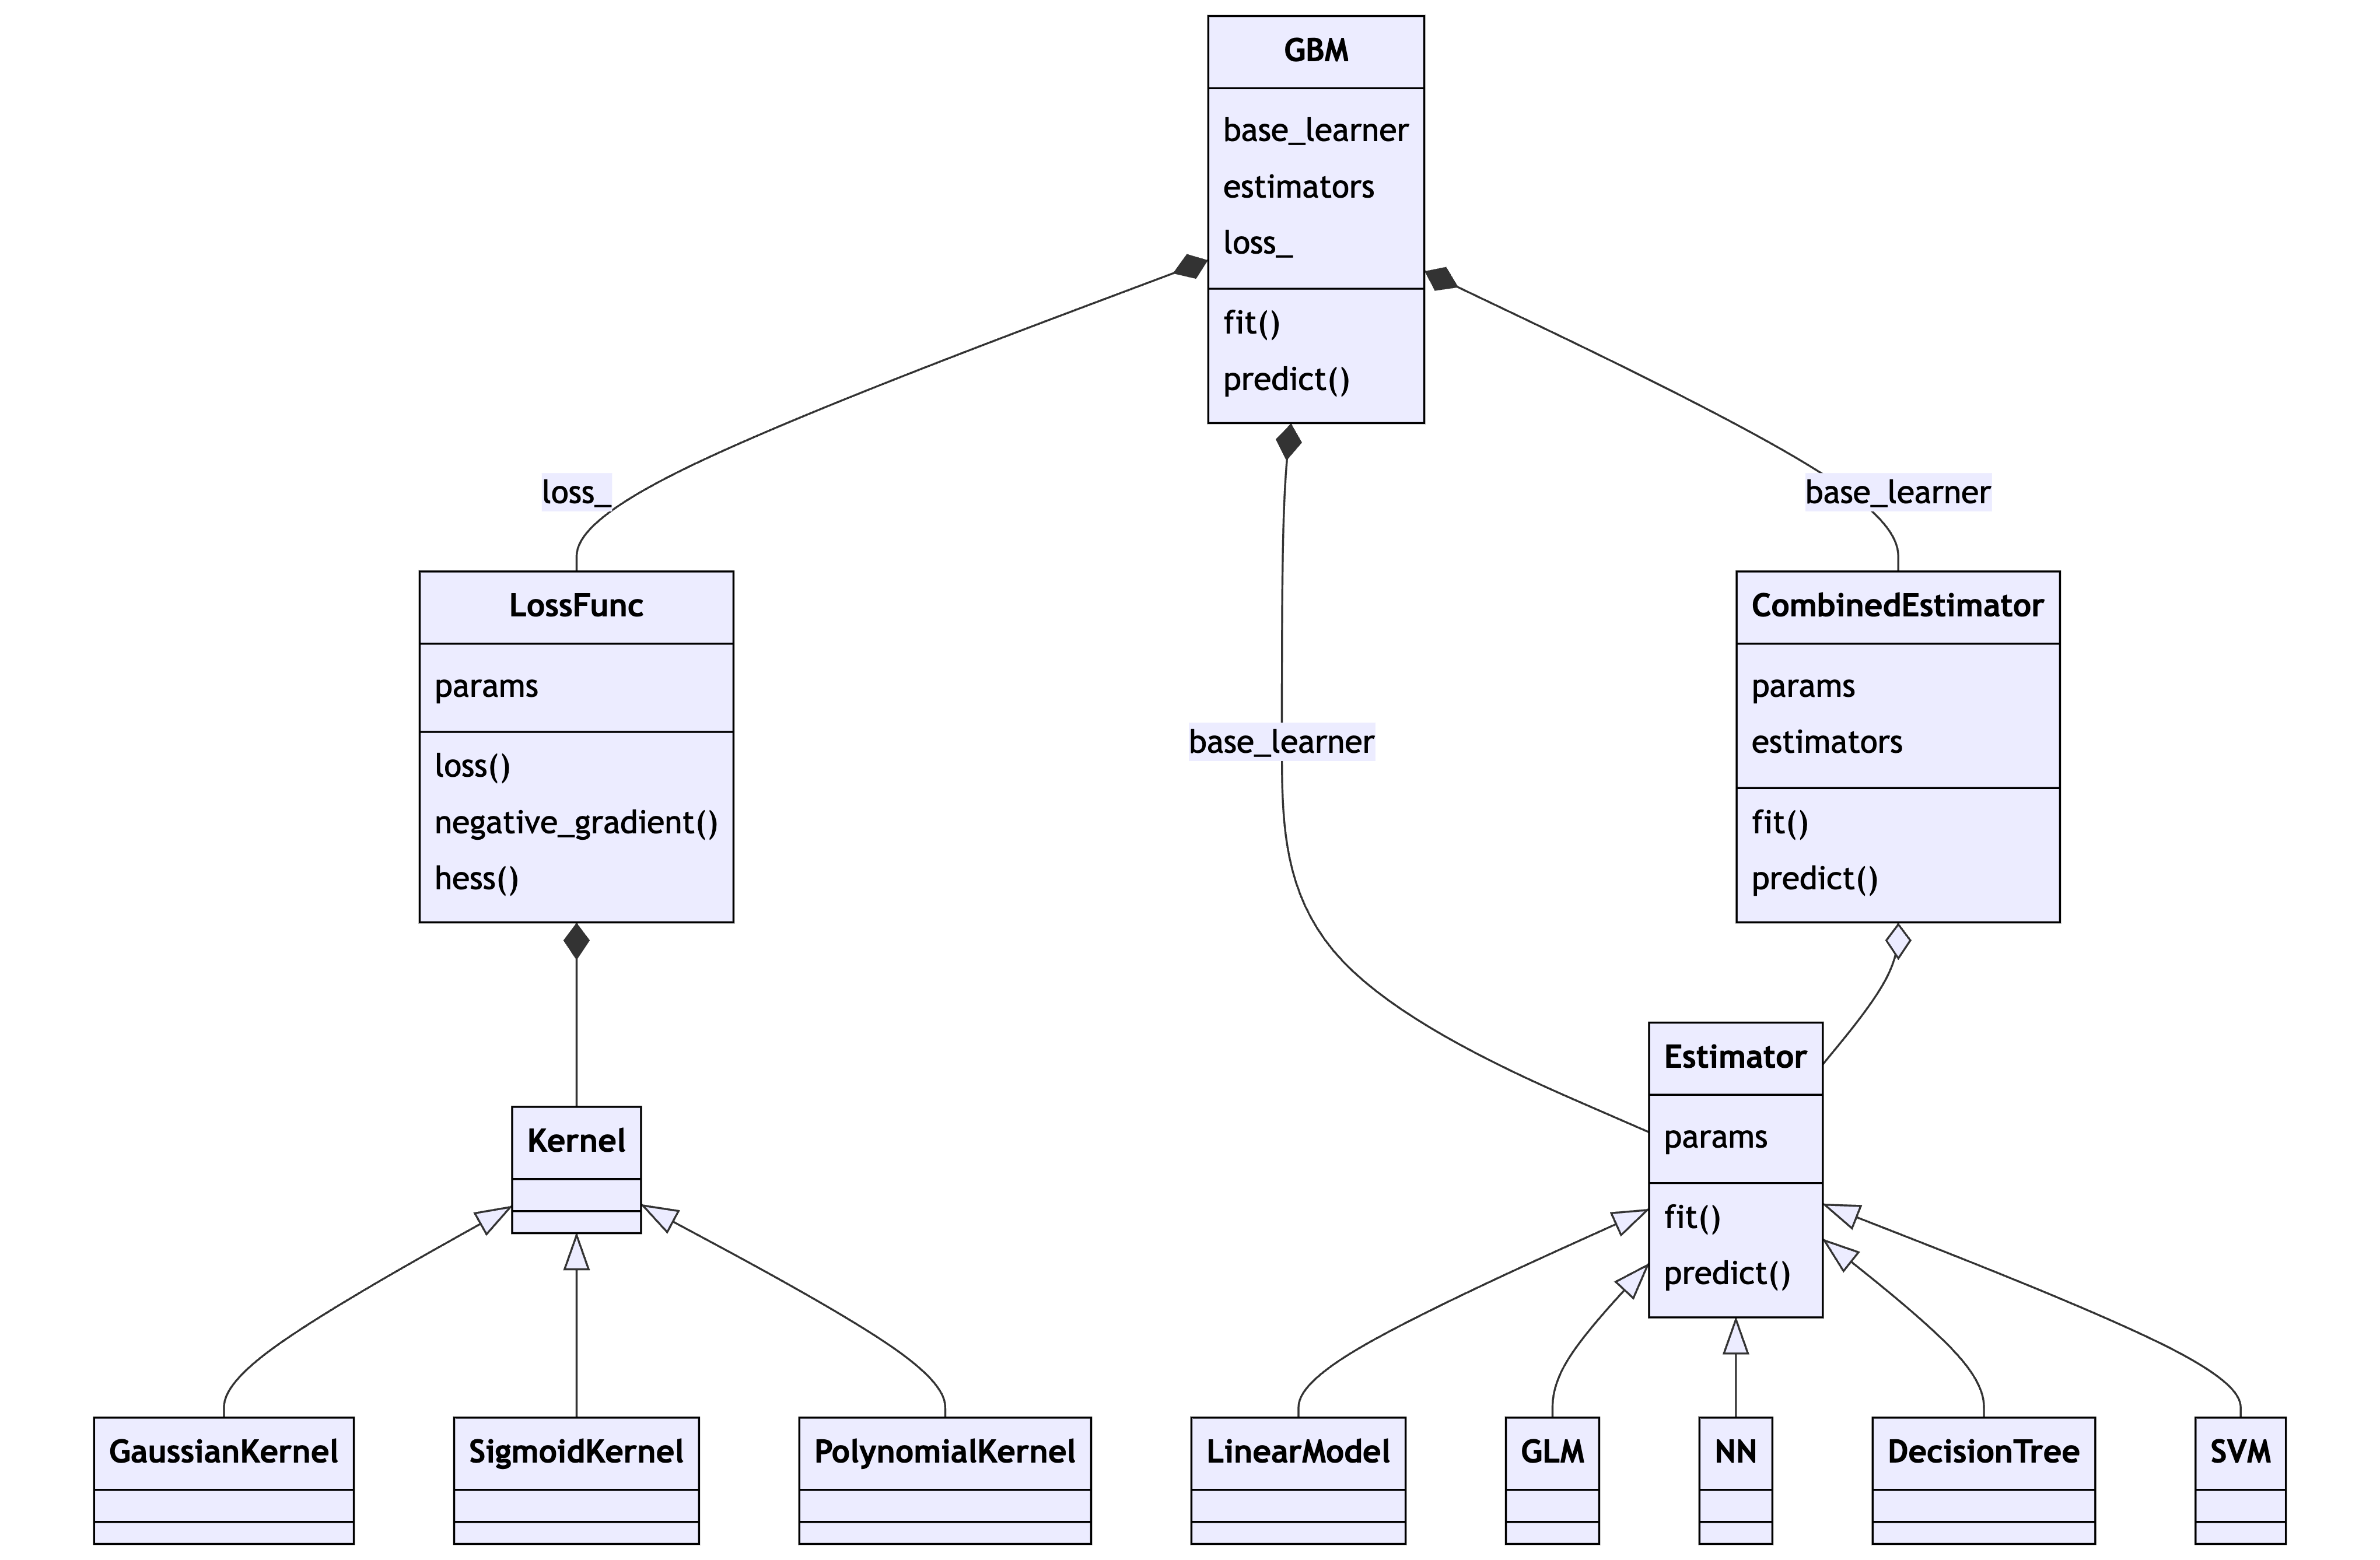
\includegraphics[height=10.5cm]{figure/rgboost.png}
	\caption{framework of rgboost}
\end{figure}
This subsection presents the RGBoost module\footnote{rgboost is available at https://github.com/nymath}. This module, based on the Python class GradientBoostingRegressor (Classifier) from the sklearn.ensemble package, is designed to yield consistent results. Unlike GradientBoostingRegressor, which restricts the base learner to decision trees, RGBoost supports the amalgamation of multiple base learners. This includes the combination function proposed by Sigrist\cite{sigrist2021ktboost}. Moreover, RGBoost integrates the gradient correction scheme proposed in this paper. One notable characteristic of our module is the versatility of the estimator class. In essence, any model with the "fit" and "negative gradient" attributes can serve as an estimator. This flexibility allows us to boost various models, such as neural networks, SVMs, GLMs, and even boosted models.Furthermore, we define the collections of different types of Estimator classes as a CombinedEstimator class. Similar to individual Estimator classes, the CombinedEstimator class also possesses "fit" and "negative gradient" attributes and, therefore, can be embedded within the GBM class.











\section{Application}
This section demonstrates the application of the gradient boosting machine to function approximation. Specifically, we employ a synthetic dataset simulated from the sinc function\footnote{See https://www.rdocumentation.org/packages/qrnn/versions/1.1.3/topics/sinc}. The simulated sinc dataset, a common benchmark for assessing regression models, comprises 200 data points evenly distributed between -10 and 10. These points are derived from a noisy sinc function, defined as sinc(x) = sin(x)/x, with Gaussian noise of mean 0 and standard deviation 0.1 added to the true function. The objective of the regression task is to learn the underlying function from this noisy data. The simulated sinc dataset serves as an effective tool for evaluating the precision and generalizability of various regression models, including gradient boosting models.

\subsection{Function Approximation}
In this subsection, we apply the revised gradient boosting machine to a simulated dataset. The sinc function dataset was divided into training and testing sets, with the model trained on the former and evaluated using the latter.

Figure \ref{fig:contrast} illustrates the results. We initially compared the performance of the Gradient Boosted Decision Trees (GBDT) on the testing set. The model leveraging the revised gradient approach (denoted by the blue curve on the learning curve) demonstrated a faster initial descent rate and lower testing error. For kernel-based learners (Gaussian kernels used for illustrative purposes), the gradient-enhanced model significantly reduced testing errors during the early iterations, but it gradually converged post-200 iterations. When we combined Reproducing Kernel Hilbert Space (RKHS) with decision trees, the testing error didn't consistently improve, which is understandable given our goal of fitting a smooth function, where the RKHS-based gradient boosting model has a natural advantage. Consequently, the combined model didn't outperform the individual models, as expected.

Figures 3 and 4 portray the model fitting process. It is evident that the revised gradient boosting algorithm (represented by the blue curve) better approximates the sample points and achieves favorable results with few iterations while maintaining other parameters constant. It's noteworthy that due to the small sample size, the model quickly begins to overfit. Moreover, when the base learner is an RKHS, the improved model can also accelerate the model's convergence speed.
\begin{figure}[htb]
	\centering
	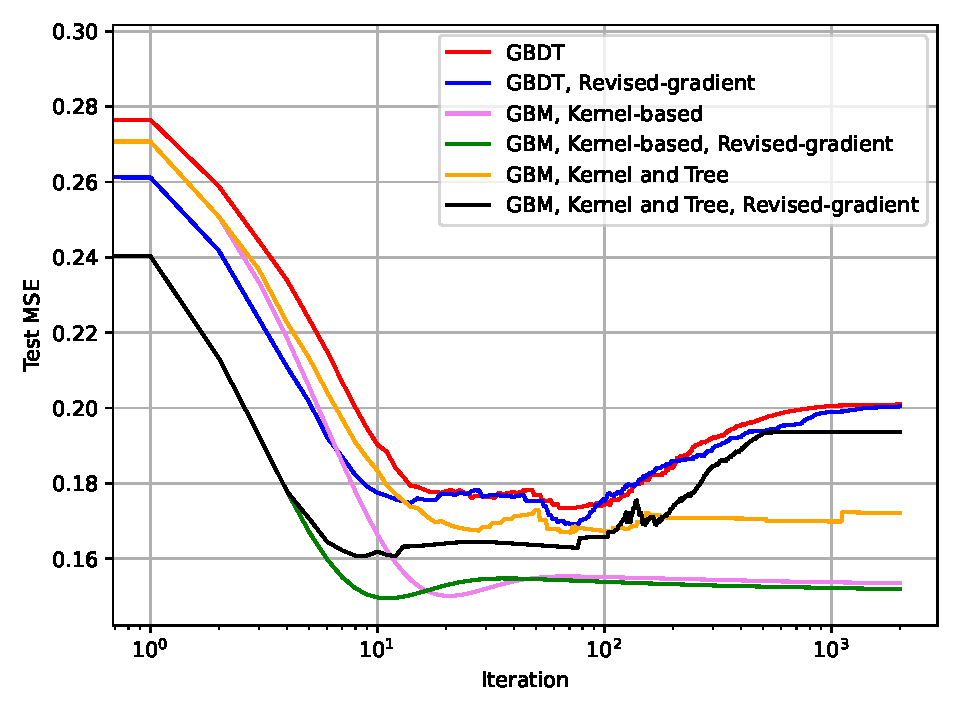
\includegraphics[height=10cm]{figure/test.pdf}
	\caption{Test MSE versus the number of iteration for comparing GBM with/without revised gradient.}
	\label{fig:contrast}
\end{figure}

\begin{figure}[htb]
	\centering
	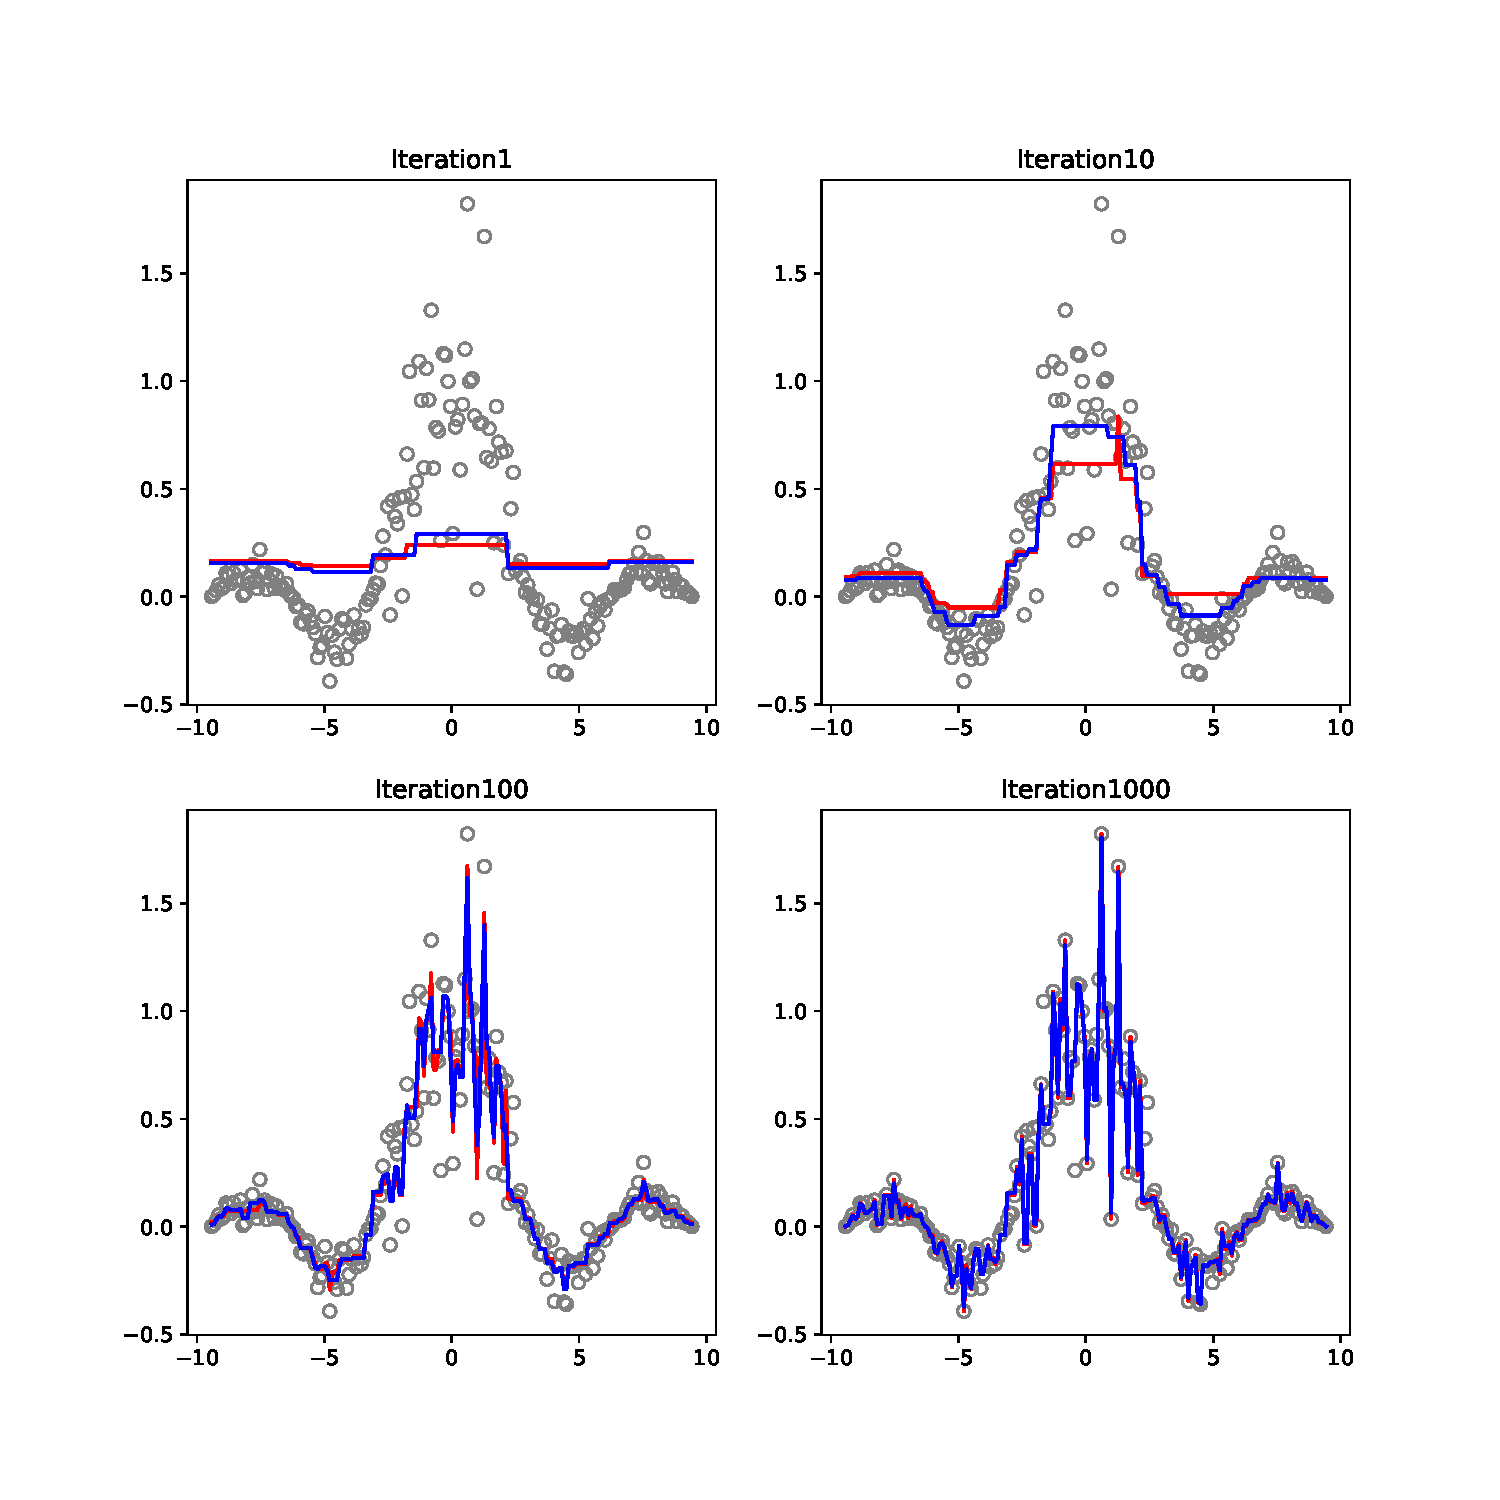
\includegraphics[height=15cm]{figure/train_process_1.pdf}
	\caption{Training process of GBDT.}
\end{figure}

\begin{figure}[htb]
	\centering
	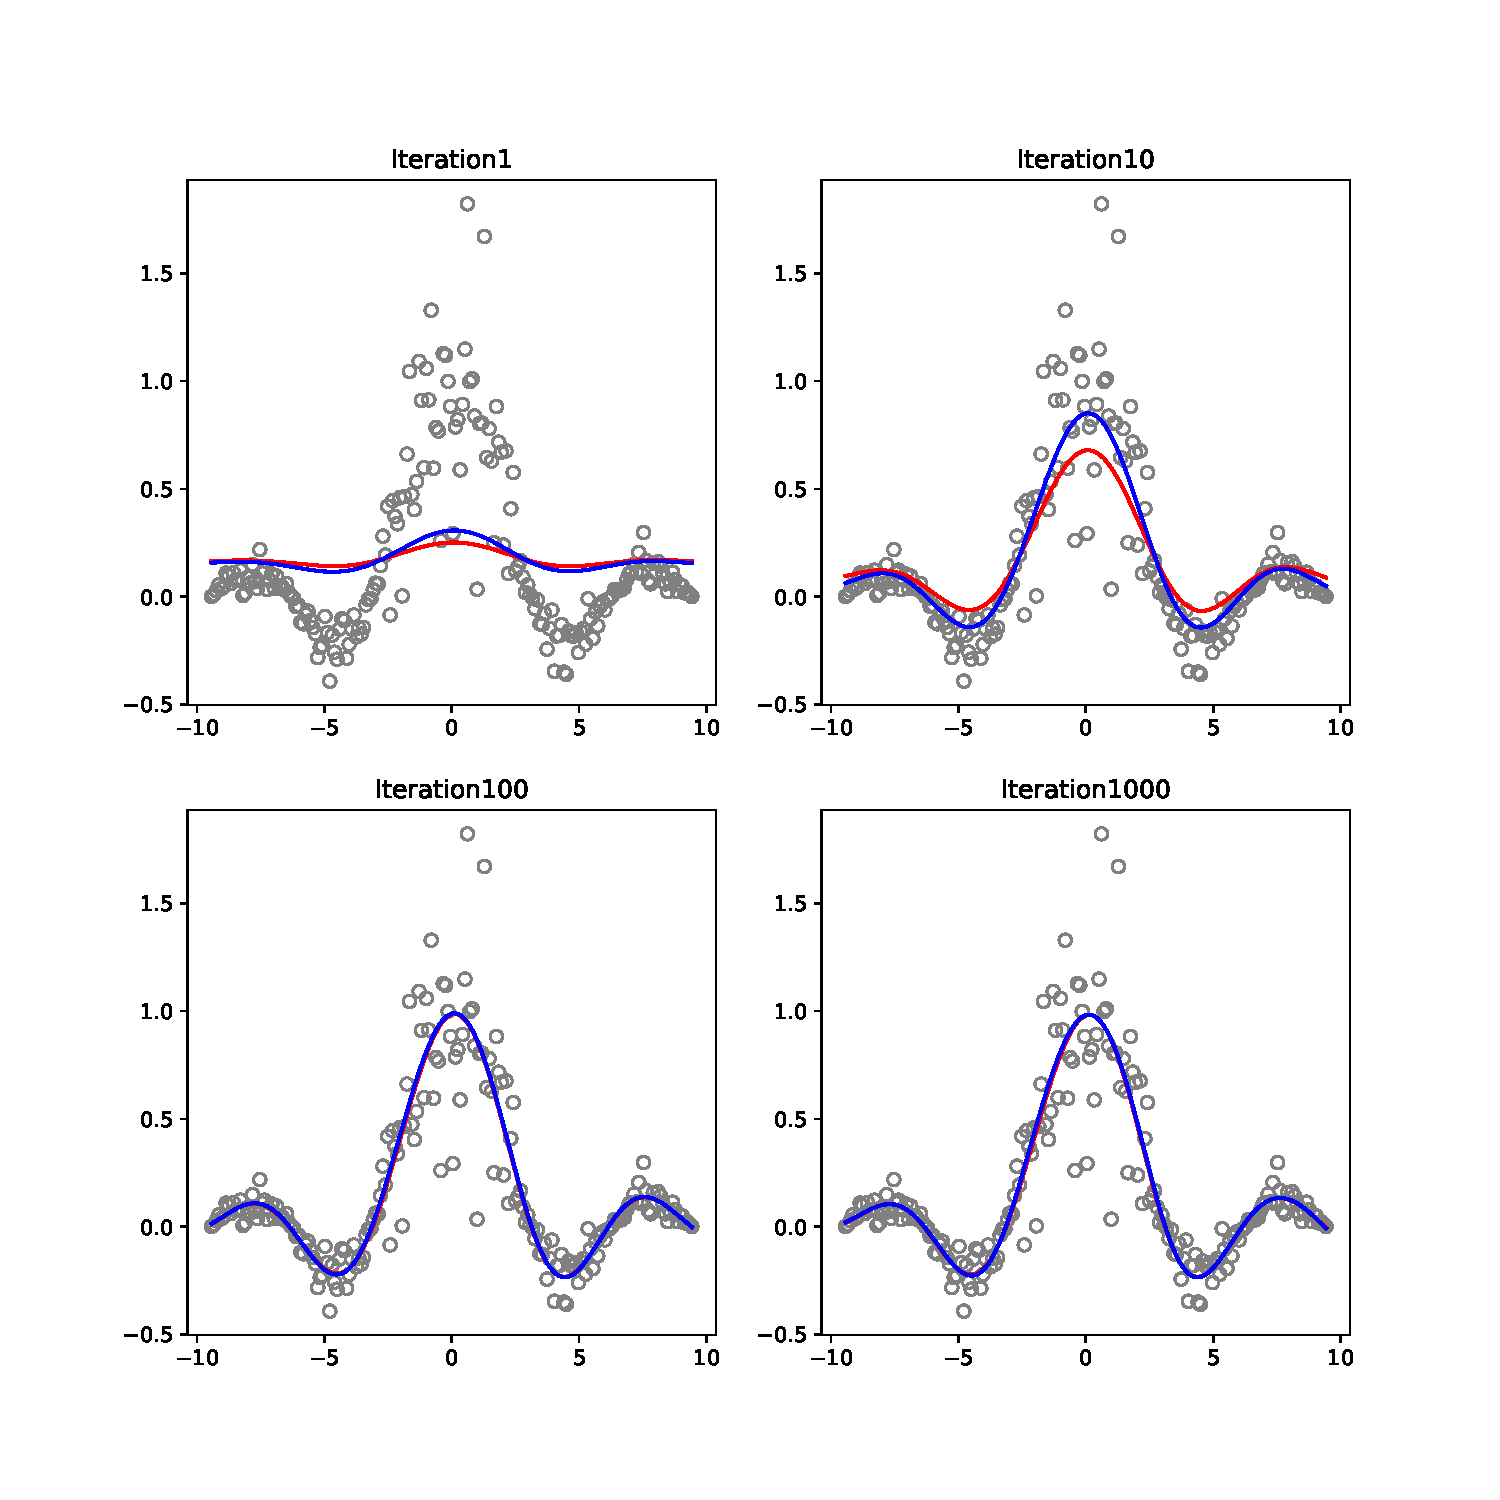
\includegraphics[height=15cm]{figure/train_process_k.pdf}
	\caption{Training process of GBM based on RKHS.}
\end{figure}





%\subsection{Event-Driven Backtesting}
%
%In this subsection, we will introduce some concepts in quantitative finance. 
%%For those who wish to learn more, we recommend visiting https://www.quantstart.com/. Established in 2012, QuantStart is an online resource for mathematical finance articles and tutorials on derivatives pricing, created to assist aspiring quants in obtaining a role in quantitative finance.
%
%There are two main frameworks in quantitative finance: vectorized backtester and event-driven backtester. While both are popular, event-driven systems provide several advantages over a vectorized approach:
%\begin{itemize}
%	
%\item \textbf{Code Reuse}: An event-driven backtester can be used for historical backtesting and live trading with minimal component switching. In contrast, vectorized backtesters require all data to be available simultaneously for statistical analysis.
%\item \textbf{Lookahead Bias}: Event-driven backtesters eliminate lookahead bias by treating market data receipt as an "event" that must be acted upon. As a result, it is possible to "drip feed" an event-driven backtester with market data, replicating how an order management and portfolio system would behave.
%\item \textbf{Realism}: Event-driven backtesters allow for significant customization over how orders are executed and transaction costs are incurred. Essential market and limit orders, as well as market-on-open (MOO) and market-on-close (MOC) orders, can be easily handled by constructing a custom exchange handler.
%\end{itemize}
%Although event-driven systems have numerous benefits, they have two significant drawbacks compared to simpler vectorized systems. Firstly, they are more complicated to implement and test due to having more "moving parts," resulting in a greater risk of introducing bugs. Proper software testing methodology, such as test-driven development, can be employed to mitigate this. Secondly, they are slower to execute than a vectorized system because optimal vectorized operations cannot be used when performing mathematical calculations. 
%
%
%Pytrade is a event-driven trading system developed us. \C{借鉴Uqer,zipline,backtesting,qstrader等多个回测框架,我编写了一个基于事件驱动的量化回测系统,还原了优矿部分 功能,极大程度的避免了量化研究中的前向偏差问题。目前该框架支持策略开发,因子投研,参数优化等功能。在下单方面, 系统充分考虑市场微观结构,支持市价单,限价单,止损单等多种订单。在事件驱动方面,系统利用事件队列的结构,能够处 理新闻数据等另类信息,并同时生成交易信号。}
%
%\begin{figure}[htb]
%\hspace{-2cm}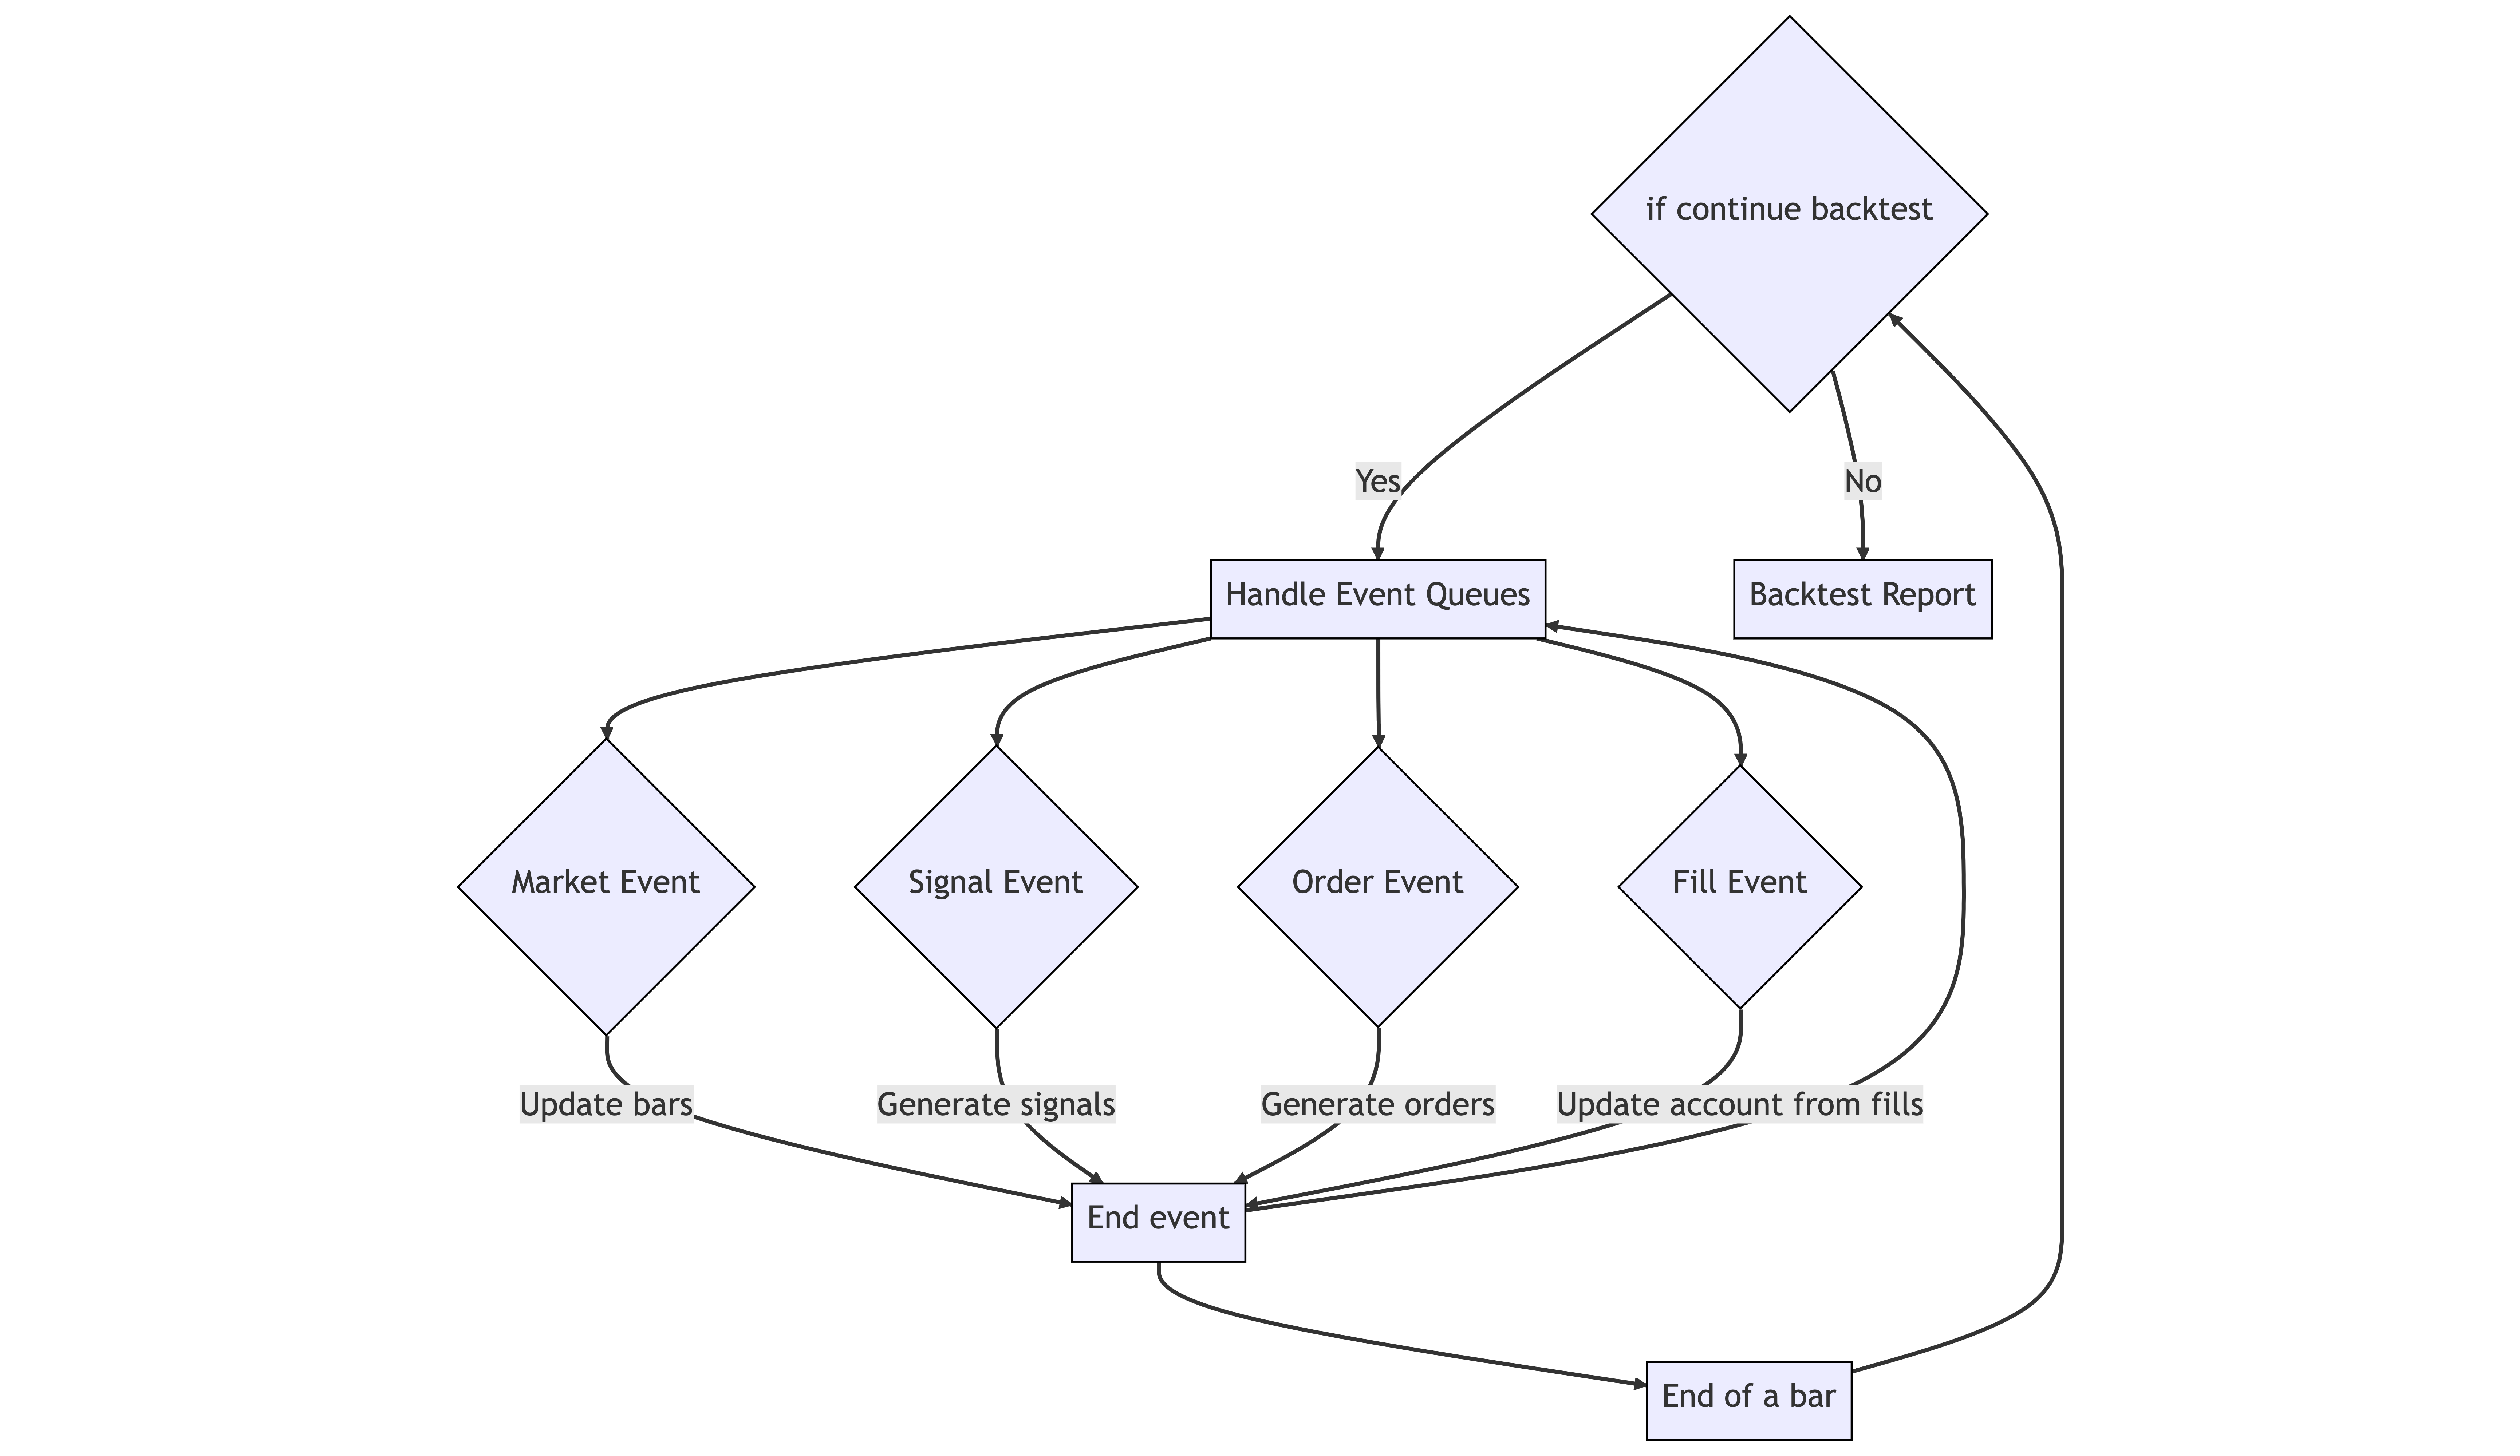
\includegraphics[scale=0.08]{figure/system.png}
%\hspace{-2cm}\caption{Event-Driven Trading System}
%\end{figure}
%




%\subsection{Stock selection based on gradient boosting}
%In stock selection, we need to choose those stocks whose price will rise significantly in the future. 
%\C{在监督学习中, 对数据进行标注至关重要, 我们按照不同的标注方式,将模型分为分类, 回归两类. 在分类问题中, 我们对股票未来一段时间内的收益率进行排序, 前百分之30标记为正, 后百分之30标记为负, }
%\begin{eqnarray*}
%B_t^{+} &=& \left\{ i: CrossQuantile(\frac{C_{t+k}^{(i)} - C_t^{(i)}}{C_t^{(i)}}) > 0.7 \right\} \\
%B_t^{-} &=& \left\{ i: CrossQuantile(\frac{C_{t+k}^{(i)} - C_t^{(i)}}{C_t^{(i)}}) < 0.3 \right\} \\
%\end{eqnarray*}
%$$
%y_t^{(i)} = \chi_{B_t^{+}}(i) -  \chi_{B_t^{-}}(i), \quad i \in B_t^+ \cup B_t^-.
%$$
%\C{而我们认为未来一段时间内收益率分位数为在0.3至0.7之间的数据为噪声, 故将其删除.}
%
%\C{风险度量指标}
%Suppose $r_t$ is the daily(hourly ...) return, then
%\begin{itemize}
%	\item Mean and Volatility 
%	$$ mean(r) = \frac{1}{T}\sum_{t=1}^{T} r_t, \quad $$
%	\item Maxdrawdown:
%	\item Sharpe Ratio:
%	\item Alpha / Excess alpha: 
%	\item Beta:
%	\vspace{1cm}
%	\item Turnover Rate:
%\end{itemize}
%
%\C{而在回归问题中, 我们就有了更多数据标注的方案.}









\section{Conclusion}

This paper presents a new gradient boosting algorithm called RGBoost, which enhances the accuracy of the gradient function approximation by modifying the negative gradient at each iteration. We define the gradient function strictly using the Riesz representation theorem and demonstrates that the gradient vector in the conventional gradient boosting algorithm is biased if the hypothesis is a Reproducing Kernel Hilbert Space (RKHS). The updated model performs significantly better than the previous model in simulated data and is subsequently applied in quantitative finance. The paper also includes an overview of related works in gradient boosting and ensemble learning, and describes the self-developed RGBoost module in Python.

\appendix
\newpage

\section{Appendix}

\subsection{Proof of Theorem \ref{thm:gradient-of-LL}}
\begin{proof}
%(theorem \ref{thm:ChainRule})
From the chain rules we have the following
\begin{eqnarray*}
	D_{\mathcal{L},f} &=& \frac{1}{n}\sum_{i=1}^n D_{L \circ E_{x_i},f} \\
	&=& \frac{1}{n}\sum_{i=1}^n D_{L,f(x_i)} \circ D_{E_{x_i},f}. \\
\end{eqnarray*} 
In addition,
\begin{eqnarray*}
	D_{\mathcal{L},f}(h) &=& \frac{1}{n}\sum_{i=1}^n D_{L,f(x_i)} \circ D_{E_{x_i},f} \circ h \\
	&=& \frac{1}{n} \sum_{i=1}^{n} \partial_2 L(y_i,f(x_i)) \inner{K_{x_i}}{h} \\
	&=& \inner{\frac{1}{n} \sum_{i=1}^{n} \partial_2 L(y_i,f(x_i)) K_{x_i}}{h}.
\end{eqnarray*}
Now the Riesz representation theorem suggests that the gradient of $\mathcal{L}$ at $f$ is the first element in the inner product notation.
\end{proof}
\subsection{Proof of Theorem \ref{thm:LS-to-RS}}
\begin{proof}
First suppose that $g \circ f$ is a simple measurable function on $\Omega$, that is 
$$
g \circ f = \sum_{k=1}^{n}c_k \chi_{F_k}, \quad F_k \in \mathcal{F}.
$$
Easy to verify that 
$$
g \circ f \circ f^{-1} = \sum_{k=1}^n c_k \chi_{f(F_k)}, 
$$
Also, we have
\begin{eqnarray*}
	\int_\R g \circ I \D \mu_f &=&  \int_\R \sum_{k=1}^n c_k \chi_{f(F_k)} \D \mu_f \\
	&=&\sum_{k=1}^n c_k \mu_f \circ f(F_k) \\
	&=& \sum_{k=1}^n c_k P \circ f^{-1} \circ f \circ F_k \\
	&=& \sum_{k=1}^n c_k P(F_k) \\
	&=& \int_{\Omega} g \circ f \D P.
\end{eqnarray*}
Since the simple-measuralbe functions are dense in $\mathcal{L}^1(\Omega,\mathcal{F},P)$, we claim that equation \ref{thm:changeofmeasure} holds if $ g \circ f \in \mathcal{L}^1(\Omega,\mathcal{F},P).$
\end{proof}


\subsection{Proof of Theorem \ref{thm:relationship}}
\begin{proof}
From theorem \ref{thm:ExistenceOfFunc} we know that $m \circ X$ is $\mathcal{F}$-measurable. Next we need to verify whether the partial average of $m \circ X$ equals to that of $Y$.
\begin{eqnarray*}
	\int_A m \circ X \D P &=& \int_\Omega \chi_A m \circ X \D P \\
	&=& \int_{\R^p} \chi_{X(A)}(x) m(x) \D \mu_X(x) \\
	&=& \int_{\R^p} \chi_{X(A)}(x) m(x) f_X(x) \D \lambda^p (x) \\
	&=& \int_{\R^p} \chi_{X(A)}(x)f_X(x) \frac{\int_\R yf(x,y) \D \lambda(y)}{f_X(x)}\D \lambda^p(x) \\
	&=& \int_{\R^p}\int_\R \chi_{X(A)}(x) y f(x,y) \D \lambda(y) \D \lambda^p(x) \\
	&=& \int_{\R^{p+1}} \chi_{X(A)}(x) y \D \mu_{X,Y}(x,y) \\
	&=& \int_A Y \D P,
\end{eqnarray*}
where the second and last equaty follows from Theorem \ref{thm:changeofmeasure}.
According to the definition of conditional expectation, we know that $m \circ X$ is the conditional expectation of $Y$ with respect to the sigma algebra generated by $X$.
\end{proof}






\section{Properties of Conditional Expectation}

\begin{Definition}[The conditional Expectation with respect a sigma-algebra] \ \\
Suppose $\MCG$ is sub-sigma-algebra of $\MCF$, $Y$ is random variable. A random variable $M$ is called the conditional expectation if 
\begin{enumerate}
	\item $M$ is $\MCG$-measurable.
	\item $\forall A \in \MCG$, $\int_A X \D P = \int_A M \D P$.  
\end{enumerate}
\end{Definition}

$M$ is often denoted by $E(X|\MCG)$.


\begin{Theorem}[Radon-Nikodym Theorem] \ \\
Suppose $\mu$ is a sigma-finite measure on a measurable space $(X,\mathcal{S})$. Suppose $\nu$ is a sigma-finite on $X, \mathcal{S}$ such that $\nu << \mu$. Then there exists $h \in \mathcal{L}^{1}(\mu)$ such that
$$
\D \nu = h \D \mu.
$$
\end{Theorem}

\begin{Definition}{The conditional Expectation with respect a random map} \ \\
Suppose $X$ is measurable map from $\Omega$ to $\mathcal{E}$(e.g. $\R^p$) and $Y$ is a random variable, then the conditional expecation of $Y$ with respect to $X$ is defined as 
$$
E(Y|X) = E(Y| X^{-1}(\mathcal{E})).
$$
\end{Definition}


\begin{Theorem}\label{thm:ExistenceOfFunc}
Suppose $X: \Omega \to E$, then $Y: \Omega \to \R$ is $\sigma(X)$-measurable if and only if there exists $h: E \to \R$, $h \in \mathcal{E}$, such that 
$$
Y = h \circ X.
$$
\end{Theorem}

%\begin{Example}
%Suppose $E \subset \R^n$, $(\Omega, \MCF, P)$ is a probability space, $X: \Omega \to E$(a random vector).
%\end{Example}




\bibliographystyle{abbrv}
\bibliography{ref}
\end{document}
